%% LyX 2.4.3 created this file.  For more info, see https://www.lyx.org/.
%% Do not edit unless you really know what you are doing.
\documentclass[journal,article,submit,pdftex,moreauthors]{Definitions/mdpi}
\usepackage[utf8]{inputenc}
\usepackage{float}
\usepackage{url}
\usepackage{bm}
\usepackage{varwidth}
\usepackage{amsmath}
\usepackage{graphicx}

\makeatletter

%%%%%%%%%%%%%%%%%%%%%%%%%%%%%% LyX specific LaTeX commands.

\Title{A novel Magnificent Frigatebird Optimization algorithm with proposed
movement strategies for enhanced Global Search}

\TitleCitation{A Novel Magnificent Frigatebird Optimization algorithm with proposed
movement strategies for enhanced Global Search}

\Author{Glykeria Kyrou$^{1}$, Vasileios Charilogis$^{2}$ and Ioannis G.
Tsoulos$^{3,*}$}

\AuthorNames{Kyrou, G., Charilogis, V., \textbackslash\& Tsoulos, I.G. }

\AuthorNames{Glykeria Kyrou, Vasileios Charilogis and Ioannis G. Tsoulos }

\AuthorCitation{Kyrou, G.; Charilogis, V.; Tsoulos, I.G.}


\address{$^{1}$\quad{}Department of Informatics and Telecommunications,
University of Ioannina, 47150 Kostaki Artas, Greece; g.kyrou@uoi.gr\\
$^{2}$\quad{}Department of Informatics and Telecommunications, University
of Ioannina, Greece; v.charilog@uoi.gr\\
$^{3}\quad$Department of Informatics and Telecommunications, University
of Ioannina, 47150 Kostaki Artas, Greece;itsoulos@uoi.gr}


\corres{Correspondence: itsoulos@uoi.gr}


\abstract{Global optimization plays a critical role in solving complex real-world
problems, where identifying the optimal solution within a high-dimensional
and nonlinear search space is essential. Metaheuristic algorithms,
inspired by natural phenomena and biological processes, have demonstrated
significant effectiveness in addressing such challenges. In this context,
the present study introduces an enhanced variant of the Magnificent
Frigatebird Optimization (MFO) algorithm, a bio-inspired metaheuristic
model that simulates the kleptoparasitic behavior of frigatebirds.
The proposed variant incorporates novel movement strategies aimed
at improving both convergence speed and solution quality. Specifically,
local search via the BFGS algorithm for refined exploitation, and
a dynamic termination criterion that detects convergence and prevents
stagnation. The algorithm is validated on an extensive set of benchmark
functions commonly found in the optimization literature, demonstrating
superior performance compared to traditional evolutionary approaches.}


\keyword{Global optimization; evolutionary methods; stochastic methods}

%% Because html converters don't know tabularnewline
\providecommand{\tabularnewline}{\\}
%% Variable width box for table cells
\newenvironment{cellvarwidth}[1][t]
    {\begin{varwidth}[#1]{\linewidth}}
    {\@finalstrut\@arstrutbox\end{varwidth}}
\floatstyle{ruled}
\newfloat{algorithm}{tbp}{loa}
\providecommand{\algorithmname}{Algorithm}
\floatname{algorithm}{\protect\algorithmname}

%%%%%%%%%%%%%%%%%%%%%%%%%%%%%% User specified LaTeX commands.
%  LaTeX support: latex@mdpi.com 
%  For support, please attach all files needed for compiling as well as the log file, and specify your operating system, LaTeX version, and LaTeX editor.

%=================================================================
%\documentclass[preprints,article,submit,pdftex,moreauthors]{Definitions/mdpi} 
% For posting an early version of this manuscript as a preprint, you may use "preprints" as the journal. Changing "submit" to "accept" before posting will remove line numbers.

% Below journals will use APA reference format:
% admsci, aichem, behavsci, businesses, econometrics, economies, education, ejihpe, famsci, games, humans, ijcs, ijfs, journalmedia, jrfm, languages, psycholint, publications, tourismhosp, youth

% Below journals will use Chicago reference format:
% arts, genealogy, histories, humanities, jintelligence, laws, literature, religions, risks, socsci

%--------------------
% Class Options:
%--------------------
%----------
% journal
%----------
% Choose between the following MDPI journals:
% accountaudit, acoustics, actuators, addictions, adhesives, admsci, adolescents, aerobiology, aerospace, agriculture, agriengineering, agrochemicals, agronomy, ai, air, algorithms, allergies, alloys, amh, analytica, analytics, anatomia, anesthres, animals, antibiotics, antibodies, antioxidants, applbiosci, appliedchem, appliedmath, appliedphys, applmech, applmicrobiol, applnano, applsci, aquacj, architecture, arm, arthropoda, arts, asc, asi, astronomy, atmosphere, atoms, audiolres, automation, axioms, bacteria, batteries, bdcc, behavsci, beverages, biochem, bioengineering, biologics, biology, biomass, biomechanics, biomed, biomedicines, biomedinformatics, biomimetics, biomolecules, biophysica, biosensors, biosphere, biotech, birds, blockchains, bloods, blsf, brainsci, breath, buildings, businesses, cancers, carbon, cardiogenetics, catalysts, cells, ceramics, challenges, chemengineering, chemistry, chemosensors, chemproc, children, chips, cimb, civileng, cleantechnol, climate, clinbioenerg, clinpract, clockssleep, cmd, cmtr, coasts, coatings, colloids, colorants, commodities, complications, compounds, computation, computers, condensedmatter, conservation, constrmater, cosmetics, covid, crops, cryo, cryptography, crystals, csmf, ctn, curroncol, cyber, dairy, data, ddc, dentistry, dermato, dermatopathology, designs, devices, diabetology, diagnostics, dietetics, digital, disabilities, diseases, diversity, dna, drones, dynamics, earth, ebj, ecm, ecologies, econometrics, economies, education, eesp, ejihpe, electricity, electrochem, electronicmat, electronics, encyclopedia, endocrines, energies, eng, engproc, ent, entomology, entropy, environments, epidemiologia, epigenomes, esa, est, famsci, fermentation, fibers, fintech, fire, fishes, fluids, foods, forecasting, forensicsci, forests, fossstud, foundations, fractalfract, fuels, future, futureinternet, futureparasites, futurepharmacol, futurephys, futuretransp, galaxies, games, gases, gastroent, gastrointestdisord, gastronomy, gels, genealogy, genes, geographies, geohazards, geomatics, geometry, geosciences, geotechnics, geriatrics, glacies, grasses, greenhealth, gucdd, hardware, hazardousmatters, healthcare, hearts, hemato, hematolrep, heritage, higheredu, highthroughput, histories, horticulturae, hospitals, humanities, humans, hydrobiology, hydrogen, hydrology, hygiene, idr, iic, ijerph, ijfs, ijgi, ijmd, ijms, ijns, ijpb, ijt, ijtm, ijtpp, ime, immuno, informatics, information, infrastructures, inorganics, insects, instruments, inventions, iot, j, jal, jcdd, jcm, jcp, jcs, jcto, jdad, jdb, jeta, jfb, jfmk, jimaging, jintelligence, jlpea, jmahp, jmmp, jmms, jmp, jmse, jne, jnt, jof, joitmc, joma, jop, jor, journalmedia, jox, jpbi, jpm, jrfm, jsan, jtaer, jvd, jzbg, kidney, kidneydial, kinasesphosphatases, knowledge, labmed, laboratories, land, languages, laws, life, lights, limnolrev, lipidology, liquids, literature, livers, logics, logistics, lubricants, lymphatics, machines, macromol, magnetism, magnetochemistry, make, marinedrugs, materials, materproc, mathematics, mca, measurements, medicina, medicines, medsci, membranes, merits, metabolites, metals, meteorology, methane, metrics, metrology, micro, microarrays, microbiolres, microelectronics, micromachines, microorganisms, microplastics, microwave, minerals, mining, mmphys, modelling, molbank, molecules, mps, msf, mti, multimedia, muscles, nanoenergyadv, nanomanufacturing, nanomaterials, ncrna, ndt, network, neuroglia, neurolint, neurosci, nitrogen, notspecified, nursrep, nutraceuticals, nutrients, obesities, oceans, ohbm, onco, oncopathology, optics, oral, organics, organoids, osteology, oxygen, parasites, parasitologia, particles, pathogens, pathophysiology, pediatrrep, pets, pharmaceuticals, pharmaceutics, pharmacoepidemiology, pharmacy, philosophies, photochem, photonics, phycology, physchem, physics, physiologia, plants, plasma, platforms, pollutants, polymers, polysaccharides, populations, poultry, powders, preprints, proceedings, processes, prosthesis, proteomes, psf, psych, psychiatryint, psychoactives, psycholint, publications, purification, quantumrep, quaternary, qubs, radiation, reactions, realestate, receptors, recycling, regeneration, religions, remotesensing, reports, reprodmed, resources, rheumato, risks, robotics, rsee, ruminants, safety, sci, scipharm, sclerosis, seeds, sensors, separations, sexes, signals, sinusitis, siuj, skins, smartcities, sna, societies, socsci, software, soilsystems, solar, solids, spectroscj, sports, standards, stats, std, stresses, surfaces, surgeries, suschem, sustainability, symmetry, synbio, systems, tae, targets, taxonomy, technologies, telecom, test, textiles, thalassrep, therapeutics, thermo, timespace, tomography, tourismhosp, toxics, toxins, transplantology, transportation, traumacare, traumas, tropicalmed, universe, urbansci, uro, vaccines, vehicles, venereology, vetsci, vibration, virtualworlds, viruses, vision, waste, water, wem, wevj, wild, wind, women, world, youth, zoonoticdis

%---------
% article
%---------
% The default type of manuscript is "article", but can be replaced by: 
% abstract, addendum, article, book, bookreview, briefreport, casereport, comment, commentary, communication, conferenceproceedings, correction, conferencereport, entry, expressionofconcern, extendedabstract, datadescriptor, editorial, essay, erratum, hypothesis, interestingimage, obituary, opinion, projectreport, reply, retraction, review, perspective, protocol, shortnote, studyprotocol, systematicreview, supfile, technicalnote, viewpoint, guidelines, registeredreport, tutorial
% supfile = supplementary materials

%----------
% submit
%----------
% The class option "submit" will be changed to "accept" by the Editorial Office when the paper is accepted. This will only make changes to the frontpage (e.g., the logo of the journal will get visible), the headings, and the copyright information. Also, line numbering will be removed. Journal info and pagination for accepted papers will also be assigned by the Editorial Office.

%------------------
% moreauthors
%------------------
% If there is only one author the class option oneauthor should be used. Otherwise use the class option moreauthors.

%---------
% pdftex
%---------
% The option pdftex is for use with pdfLaTeX. If eps figures are used, remove the option pdftex and use LaTeX and dvi2pdf.

%=================================================================
% MDPI internal commands - do not modify
\firstpage{1} 
\setcounter{page}{\@firstpage}
\pubvolume{1}
\issuenum{1}
\articlenumber{0}
\pubyear{2025}
\copyrightyear{2025}
%\externaleditor{Firstname Lastname} % More than 1 editor, please add `` and '' before the last editor name
\datereceived{}
\daterevised{ } % Comment out if no revised date
\dateaccepted{}
\datepublished{}
%\datecorrected{} % For corrected papers include a "Corrected: XXX" date in the original paper.
%\dateretracted{} % For retracted papers include a "RETRACTED: XXX" date in the original paper.
\hreflink{https://doi.org/} % If needed use \linebreak
%\doinum{}
%\pdfoutput=1 % Uncommented for upload to arXiv.org
%\CorrStatement{yes}  % For updates
%\longauthorlist{yes} % For many authors that exceed the left citation part

%=================================================================
% Add packages and commands here. The following packages are loaded in our class file: fontenc, inputenc, calc, indentfirst, fancyhdr, graphicx, epstopdf, lastpage, ifthen, lineno, float, amsmath, setspace, enumitem, mathpazo, booktabs, titlesec, etoolbox, tabto, xcolor, soul, multirow, microtype, tikz, totcount, changepage, attrib, upgreek, cleveref, amsthm, hyphenat, natbib, hyperref, footmisc, url, geometry, newfloat, caption

%=================================================================
%% Please use the following mathematics environments: Theorem, Lemma, Corollary, Proposition, Characterization, Property, Problem, Example, ExamplesandDefinitions, Hypothesis, Remark, Definition, Notation, Assumption
%% For proofs, please use the proof environment (the amsthm package is loaded by the MDPI class).

%=================================================================
% The fields PACS, MSC, and JEL may be left empty or commented out if not applicable
%\PACS{J0101}
%\MSC{}
%\JEL{}

%%%%%%%%%%%%%%%%%%%%%%%%%%%%%%%%%%%%%%%%%%
% Only for the journal Diversity
%\LSID{\url{http://}}

%%%%%%%%%%%%%%%%%%%%%%%%%%%%%%%%%%%%%%%%%%
% Only for the journal Applied Sciences:
%\featuredapplication{Authors are encouraged to provide a concise description of the specific application or a potential application of the work. This section is not mandatory.}
%%%%%%%%%%%%%%%%%%%%%%%%%%%%%%%%%%%%%%%%%%

%%%%%%%%%%%%%%%%%%%%%%%%%%%%%%%%%%%%%%%%%%
% Only for the journal Data:
%\dataset{DOI number or link to the deposited data set in cases where the data set is published or set to be published separately. If the data set is submitted and will be published as a supplement to this paper in the journal Data, this field will be filled by the editors of the journal. In this case, please make sure to submit the data set as a supplement when entering your manuscript into our manuscript editorial system.}

%\datasetlicense{license under which the data set is made available (CC0, CC-BY, CC-BY-SA, CC-BY-NC, etc.)}

%%%%%%%%%%%%%%%%%%%%%%%%%%%%%%%%%%%%%%%%%%
% Only for the journal BioTech, Fishes, Neuroimaging and Toxins
%\keycontribution{The breakthroughs or highlights of the manuscript. Authors can write one or two sentences to describe the most important part of the paper.}

%%%%%%%%%%%%%%%%%%%%%%%%%%%%%%%%%%%%%%%%%%
% Only for the journal Encyclopedia
%\encyclopediadef{Instead of the abstract}
%\entrylink{The Link to this entry published on the encyclopedia platform.}
%%%%%%%%%%%%%%%%%%%%%%%%%%%%%%%%%%%%%%%%%%

%%%%%%%%%%%%%%%%%%%%%%%%%%%%%%%%%%%%%%%%%%
% Different journals have different requirements. Please check the specific journal guidelines in the "Instructions for Authors" on the journal's official website.
 
%\addhighlights{yes}
%\renewcommand{\addhighlights}{%
%
%\noindent The goal is to increase the discoverability and readability of the article via search engines and other scholars. Highlights should not be a copy of the abstract, but a simple text allowing the reader to quickly and simplified find out what the article is about and what can be cited from it. Each of these parts should be devoted up to 2 bullet points.\vspace{3pt}\\
%\textbf{What are the main findings?}
% \begin{itemize}[labelsep=2.5mm,topsep=-3pt]
% \item First bullet.
% \item Second bullet.
% \end{itemize}\vspace{3pt}
%\textbf{What is the implication of the main finding?}
% \begin{itemize}[labelsep=2.5mm,topsep=-3pt]
% \item First bullet.
% \item Second bullet.
% \end{itemize}
%}
%%%%%%%%%%%%%%%%%%%%%%%%%%%%%%%%%%%%%%%%%%

\makeatother

\begin{document}
\maketitle

\section{Introduction}

The primary objective of global optimization is to locate the global
minimum of a continuous and multidimensional function, in such a way
as to ensure complete exploration of the search space. Global optimization
aims to examine the entire problem domain in order to find the lowest
possible value that is feasible. This procedure is applied to complex
functions which usually include multiple local minima, making it difficult
to identify the global minimum. Global optimization includes techniques
that ensure that local optima are avoided while focusing on maximizing
the accuracy and efficiency of the search process. The objective is
to find the lowest point through systematic exploration of the entire
domain of the function$f:S\rightarrow R,S\subset R^{n}$ and it is
defined as follows:

\begin{equation}
x^{*}=\mbox{arg}\min_{x\in S}f(x)\label{eq:eq1-1}
\end{equation}
where the set $S$ is defined as follows: 
\[
S=\left[a_{1},b_{1}\right]\times\left[a_{2},b_{2}\right]\times\ldots\left[a_{n},b_{n}\right]
\]

Global optimization constitutes one of the most dynamically evolving
fields of applied mathematical analysis and computer science, as it
seeks the discovery of the globally optimal solution to problems characterized
by high complexity, large dimensionality, and strong nonlinearity.
In contrast to local methods, which identify solutions within limited
regions of the search space, global optimization techniques aim to
explore the entire search domain, thus providing solutions of validated
quality. During the recent years, a magnitude of reviews for this
problem have been published by various researchers \citep{go1,go2,go3}.
Their significance is not merely theoretical; they find direct application
in critical scientific disciplines such as mathematics \citep{go_math1,go_math3},
physics \citep{go_physics2,go_physics3}, chemistry \citep{go_chem1,go_chem2},
medicine \citep{go_med2,medicine} and economics \citep{key-1,go_econ2}
where the requirements for accuracy and reliability are particularly
demanding.

In this research area, two main approaches have been established:
deterministic \citep{key-2,go_determ3} and stochastic methods \citep{stohastic,stohastic1}.
Deterministic techniques are grounded in rigorous mathematical foundations
and provide theoretical guarantees for locating the global minimum.
A characteristic example is interval analysis methods, which pursue
the gradual subdivision of the search space until regions of increased
interest are identified. Despite their accuracy, their high computational
cost restricts their applicability to relatively small-scale problems.
In contrast, stochastic methods, although lacking a mathematical guarantee
of finding the optimal solution, demonstrate considerable flexibility
in highly complex environments. Representative examples include Controlled
Random Search \citep{crs1,crs2}, Simulated Annealing \citep{simann_major,simann1},
and Multistart \citep{mult_minfinder,mult_cfo}, which, however, encounter
difficulties when strong nonlinear constraints are involved.

Within the framework of stochastic approaches, particular importance
is attributed to evolutionary computation, which draws inspiration
from the principles of biological evolution and natural selection.
Its central idea is that the mechanisms of adaptation and survival
observed in nature can be modeled computationally, providing powerful
tools for solving large-scale and highly complex problems. This category
includes Genetic Algorithms \citep{key-3,genetic3}, Evolution Strategies
\citep{key-9,key-10}, Genetic Programming \citep{key-11,key-12},
and Differential Evolution (DE) \citep{diffe1,diffe2}. At the same
time, related stochastic methods include approaches inspired by the
collective behavior of biological systems, such as Particle Swarm
Optimization (PSO) \citep{pso_major,pso1} and Ant Colony Optimization
(ACO)\citep{aco1,aco2}. 

In recent years, research has increasingly focused on more specialized
bio-inspired algorithms, which attempt to capture even more distinctive
behaviors observed in the natural world. A representative example
is the Magnificent Frigatebird Optimization (MFO) algorithm \citep{key-16},
which is based on the study of the frigatebird, a large seabird found
in tropical and subtropical regions of the Americas. This species
is notable for its kleptoparasitic foraging strategy: rather than
hunting independently, it attacks other seabirds, forces them to drop
their prey, and then swiftly dives to seize it before it sinks into
the sea. This adaptive and highly effective behavior has served as
the basis for the mathematical design of MFO, in which the notion
of “attacking competitors to acquire resources” is translated into
mechanisms of exploration and exploitation within the solution space.
In this way, MFO is incorporated into the rapidly expanding family
of bio-inspired algorithms, enriching the field of global optimization
with innovative strategies.

The current work introduces a series of modifications to the MFO algorithm,
in order to speed up the process and increase the efficiency of the
algorithm. These modifications include:
\begin{itemize}
\item \textbf{Three movement strategies:}
\begin{itemize}
\item The aggressive strategy focuses on intense movement towards better
candidates, enhancing the exploration ability.
\item The conservative strategy is oriented in smaller steps around the
best solution so far, promoting exploitation.
\item The mixed strategy combines the characteristics of the two previous
ones, ensuring a more balanced behavior of the algorithm.
\end{itemize}
\item Furthermore, \textbf{local search} was incorporated through the BFGS
algorithm\citep{Powell} with the aim of refining candidate solutions
and improving convergence towards optimal points.
\item Finally, an early\textbf{ termination technique}\citep{stopping rule2}
based on stochastic observations was applied. At each iteration of
the algorithm, the optimal value of the objective function up to that
moment is recorded. If this value remains unchanged for a predetermined
number of iterations, the optimization process is stopped. In this
way, unnecessary execution of further calculations is avoided when
no substantial progress is observed, leading to a more efficient use
of computational time.
\end{itemize}
The remains of this paper are divided as follows: in section\ref{sec:Materials-and-Methods}
the proposed MFO algorithm, a flowchart with a detailed description
is presented, in section\ref{sec:Results} of the test functions used
in the experiments as well as the related experiments are presented.
In the \ref{sec:Discussion}section, there is a brief discussion of
the results obtained from the experiments. In section \ref{sec:Conclusions}some
conclusions and directions for future improvements are discussed.

\section{Materials and Methods\label{sec:Materials-and-Methods}}

\subsection{The main steps of the algorithm}

The Magnificent Frigatebird (MFO) optimization algorithm is a metaheuristic
algorithm inspired by biology. It combines the cooperative foraging
behavior of magnificent frigatebirds in a marine environment. Each
agent represents a frigate that explores the search space looking
for better food sources, i.e. the best solutions to the optimization
problem. The algorithm starts by initializing a population of candidate
solutions and evaluating their performance. The best individual is
then recorded.

During each generation, the agents are evaluated, and a subset may
undergo local search to refine their positions and improve accuracy
before the population is ranked according to fitness. The search process
alternates between two phases: the exploration phase, where agents
perform adaptive movements to discover new and promising regions of
the search space, and the exploitation phase, where they focus on
refining the best solutions found so far to enhance precision and
convergence. These two behaviors are expressed through\textbf{ aggressive},
\textbf{conservative}, or \textbf{mixed} \textbf{strategies}, allowing
a dynamic balance between global exploration and local intensification
throughout the optimization process.

At the end of each generation, the best solution can be further improved
through a local optimization step to enhance convergence accuracy.
The process continues until a termination criterion, such as the maximum
number of generations or population convergence, is met. The final
result represents the best solution found. In conclusion, the MFO
algorithm achieves a strong balance between exploration and exploitation
through adaptive tuning and selective improvement, providing satisfactory
performance on a range of different optimization problems. The steps
of the Magnificent Frigatebird Optimization (MFO) algorithm presented
in Algorithm \ref{alg:Magnificent-Frigatebird-Optimiza}.

\begin{algorithm}
\caption{Magnificent Frigatebird Optimization (MFO) algorithm\label{alg:Magnificent-Frigatebird-Optimiza}}

{\scriptsize\textbf{INPUT}}{\scriptsize\par}

{\scriptsize - $N$: population size. }{\scriptsize\par}

{\scriptsize - $G_{\mbox{max}}$: max generations.}{\scriptsize\par}

{\scriptsize - $T$: inner iterations per generation.}{\scriptsize\par}

{\scriptsize - $\mbox{strategyMode\ensuremath{\in}\ensuremath{\left\{  \mbox{aggresive},\mbox{conservative,\mbox{mixed}}\right\} } }$.}{\scriptsize\par}

{\scriptsize - $p_{l}\in[0,1]$ as the local search rate.}{\scriptsize\par}

{\scriptsize\textbf{OUTPUT}}{\scriptsize\par}

{\scriptsize -$\left(x_{\mbox{best}},f_{\mbox{best}}\right)$}{\scriptsize\par}

{\scriptsize\textbf{INITIALIZATION}}{\scriptsize\par}

{\scriptsize - }{\scriptsize\textbf{Sample}}{\scriptsize{} initial population
$P$ of size $N$ uniformly in $S$ and evaluate $f$}{\scriptsize\par}

{\scriptsize - }{\scriptsize\textbf{Obtain}}{\scriptsize{} the current
best $\left(x_{\mbox{best}},f_{\mbox{best}}\right)$ from $P$}{\scriptsize\par}

{\scriptsize - }{\scriptsize\textbf{Set}}{\scriptsize{} $k=0$, the generation
counter.}{\scriptsize\par}

{\scriptsize\textbf{MFO main pseudocode }}{\scriptsize\par}

{\scriptsize 01}{\scriptsize\textbf{ while}}{\scriptsize{} $k<G_{\mbox{max}}$
and the termination rule described in subsection \ref{subsec:The-used-termination}
does not hold }{\scriptsize\textbf{do}}{\scriptsize\par}

{\scriptsize 02 \hspace{0.5cm}}{\scriptsize\textbf{Set}}{\scriptsize{}
$k=k+1$}{\scriptsize\par}

{\scriptsize 03 \hspace{0.5cm}}{\scriptsize\textbf{for}}{\scriptsize{}
$i=1,\ldots,N$ }{\scriptsize\textbf{do}}{\scriptsize\par}

{\scriptsize 04 \hspace{0.5cm}\hspace{0.5cm}$f_{i}=f\left(P_{i}\right)$}{\scriptsize\par}

{\scriptsize 05 \hspace{0.5cm}\hspace{0.5cm}Pick a random number
$r\in[0,1]$.}{\scriptsize\par}

{\scriptsize 06 \hspace{0.5cm}\hspace{0.5cm}}{\scriptsize\textbf{If}}{\scriptsize{}
$r\le p_{l}$ }{\scriptsize\textbf{then}}{\scriptsize{} $f_{i}=\mbox{LS}(P_{i})$,
Where $\mbox{LS}(x)$ is a local optimization procedure. }{\scriptsize\par}

{\scriptsize 07 \hspace{0.5cm}}{\scriptsize\textbf{endfor}}{\scriptsize\par}

{\scriptsize 08\hspace{0.5cm}}{\scriptsize\textbf{ Obtain}}{\scriptsize{}
the current best $\left(x_{\mbox{best}},f_{\mbox{best}}\right)$ from
$P$}{\scriptsize\par}

{\scriptsize 09 \hspace{0.5cm}sort $P$ according to the fitness values.}{\scriptsize\par}

{\scriptsize 10 \hspace{0.5cm}}{\scriptsize\textbf{for}}{\scriptsize{}
$t=1,\ldots,T$}{\scriptsize\textbf{ do}}{\scriptsize\par}

{\scriptsize 11 \hspace{0.5cm}\hspace{0.5cm}}{\scriptsize\textbf{for}}{\scriptsize{}
$i=1,\ldots,N$ }{\scriptsize\textbf{do}}{\scriptsize\par}

{\scriptsize 12 \hspace{0.5cm}\hspace{0.5cm}\hspace{0.5cm}// Phase
A: move using better “seabird” or best, depending on strategyMode}{\scriptsize\par}

{\scriptsize 13 \hspace{0.5cm}\hspace{0.5cm}\hspace{0.5cm}}{\scriptsize\textbf{Set
}}{\scriptsize$C=\left\{ P_{k}:k\ne i\ \mbox{and}\ f\left(P_{k}\right)<f\left(P_{i}\right)\right\} $ }{\scriptsize\par}

{\scriptsize 14 \hspace{0.5cm}\hspace{0.5cm}\hspace{0.5cm}}{\scriptsize\textbf{Pick}}{\scriptsize{}
$SS$ a random element of $C$}{\scriptsize\par}

{\scriptsize 15 \hspace{0.5cm}\hspace{0.5cm}\hspace{0.5cm}}{\scriptsize\textbf{if}}{\scriptsize{}
$\mbox{strategyMode}=\mbox{aggresive}$ }{\scriptsize\textbf{then}}{\scriptsize\par}

{\scriptsize 16 \hspace{0.5cm}\hspace{0.5cm}\hspace{0.5cm}\hspace{0.5cm}}{\scriptsize\textbf{for}}{\scriptsize{}
$j=1,\ldots,n$ }{\scriptsize\textbf{do}}{\scriptsize\par}

{\scriptsize 17 \hspace{0.5cm}\hspace{0.5cm}\hspace{0.5cm}\hspace{0.5cm}\hspace{0.5cm}}{\scriptsize\textbf{Pick}}{\scriptsize{}
a random number $r\in[0,1]$.}{\scriptsize\par}

{\scriptsize 18 \hspace{0.5cm}\hspace{0.5cm}\hspace{0.5cm}\hspace{0.5cm}\hspace{0.5cm}}{\scriptsize\textbf{Set}}{\scriptsize{}
$I\in\left\{ 1,2\right\} $ a random integer value.}{\scriptsize\par}

{\scriptsize 19 \hspace{0.5cm}\hspace{0.5cm}\hspace{0.5cm}\hspace{0.5cm}\hspace{0.5cm}}{\scriptsize\textbf{Set
}}{\scriptsize$y_{j}=P_{i,j}+2(r-0.5)\left(SS_{j}-IP_{i,j}\right)$}{\scriptsize\par}

{\scriptsize 20 \hspace{0.5cm}\hspace{0.5cm}\hspace{0.5cm}\hspace{0.5cm}}{\scriptsize\textbf{endfor}}{\scriptsize\par}

{\scriptsize 21 \hspace{0.5cm}\hspace{0.5cm}\hspace{0.5cm}}{\scriptsize\textbf{else
if}}{\scriptsize{} strategyMode = conservative }{\scriptsize\textbf{then}}{\scriptsize\par}

{\scriptsize 22 \hspace{0.5cm}\hspace{0.5cm}\hspace{0.5cm}\hspace{0.5cm}}{\scriptsize\textbf{for}}{\scriptsize{}
$j=1,\ldots,n$ }{\scriptsize\textbf{do}}{\scriptsize\par}

{\scriptsize 23 \hspace{0.5cm}\hspace{0.5cm}\hspace{0.5cm}\hspace{0.5cm}\hspace{0.5cm}}{\scriptsize\textbf{Set}}{\scriptsize{}
$r\in[0,1]$ a randomly selected number.}{\scriptsize\par}

{\scriptsize 24 \hspace{0.5cm}\hspace{0.5cm}\hspace{0.5cm}\hspace{0.5cm}\hspace{0.5cm}}{\scriptsize\textbf{Set
}}{\scriptsize$y_{j}=P_{i,j}+0.3\left(r-0.5\right)\left(x_{best,j}-P_{i,j}\right)$}{\scriptsize\par}

{\scriptsize 25 \hspace{0.5cm}\hspace{0.5cm}\hspace{0.5cm}\hspace{0.5cm}}{\scriptsize\textbf{endfor}}{\scriptsize\par}

{\scriptsize 26 \hspace{0.5cm}\hspace{0.5cm}\hspace{0.5cm}}{\scriptsize\textbf{else}}{\scriptsize{}
// mixed strategy}{\scriptsize\par}

{\scriptsize 27 \hspace{0.5cm}\hspace{0.5cm}\hspace{0.5cm}\hspace{0.5cm}}{\scriptsize\textbf{Select}}{\scriptsize{}
with probability 50\% the aggressive or the conservative strategy.}{\scriptsize\par}

{\scriptsize 28 \hspace{0.5cm}\hspace{0.5cm}\hspace{0.5cm}}{\scriptsize\textbf{endif}}{\scriptsize\par}

{\scriptsize 29 \hspace{0.5cm}\hspace{0.5cm}\hspace{0.5cm}}{\scriptsize\textbf{if}}{\scriptsize{}
$y\ \in\ S$ and $f(y)<f\left(P_{i}\right)$ }{\scriptsize\textbf{then}}{\scriptsize\par}

{\scriptsize 30 \hspace{0.5cm}\hspace{0.5cm}\hspace{0.5cm}\hspace{0.5cm}}{\scriptsize\textbf{Set
}}{\scriptsize$P_{i}=y$}{\scriptsize\par}

{\scriptsize 31 \hspace{0.5cm}\hspace{0.5cm}\hspace{0.5cm}}{\scriptsize\textbf{endif}}{\scriptsize\par}

{\scriptsize 32 \hspace{0.5cm}\hspace{0.5cm}}{\scriptsize\textbf{endif}}{\scriptsize\par}

{\scriptsize 33 \hspace{0.5cm}\hspace{0.5cm}// Phase B (dive): pull
towards current best solution}{\scriptsize\par}

{\scriptsize 34 \hspace{0.5cm}\hspace{0.5cm}}{\scriptsize\textbf{Set}}{\scriptsize{}
$b=\arg\min_{k}f\left(P_{k}\right)$ // bestSolution in population
after Phase A}{\scriptsize\par}

{\scriptsize 35 \hspace{0.5cm}\hspace{0.5cm}}{\scriptsize\textbf{for}}{\scriptsize{}
$j=1,\ldots,n$ }{\scriptsize\textbf{do}}{\scriptsize\par}

{\scriptsize 36 \hspace{0.5cm}\hspace{0.5cm}\hspace{0.5cm}}{\scriptsize\textbf{Set
$r\in[0,1]$ }}{\scriptsize a randomly selected number }{\scriptsize\par}

{\scriptsize 37 \hspace{0.5cm}\hspace{0.5cm}\hspace{0.5cm}Set $z_{j}=P_{i,j}+\left(1-2r\right)\left(b_{j}-\frac{P_{i,j}}{t}\right)$}{\scriptsize\par}

{\scriptsize 38 \hspace{0.5cm}\hspace{0.5cm}}{\scriptsize\textbf{if}}{\scriptsize{}
$z\in S$ and $f\left(z\right)<f_{i}$ }{\scriptsize\textbf{then set
$P_{i}=z$}}{\scriptsize\par}

{\scriptsize 39 \hspace{0.5cm}\hspace{0.5cm}}{\scriptsize\textbf{endfor}}{\scriptsize\par}

{\scriptsize 40 \hspace{0.5cm}}{\scriptsize\textbf{endfor}}{\scriptsize\par}

{\scriptsize 41 \hspace{0.5cm}}{\scriptsize\textbf{Set}}{\scriptsize{}
$f_{\mbox{best}}=\mbox{LS}\left(x_{\mbox{best}}\right)$}{\scriptsize\par}

{\scriptsize 42 }{\scriptsize\textbf{endwhile}}{\scriptsize\par}

{\scriptsize 43 }{\scriptsize\textbf{return}}{\scriptsize{} $\left(x_{\mbox{best}},f_{\mbox{best}}\right)$}{\scriptsize\par}
\end{algorithm}
 Furthermore, the steps of the proposed method are also graphically
shown in Figure \ref{fig:Algorithm}.

\begin{figure}
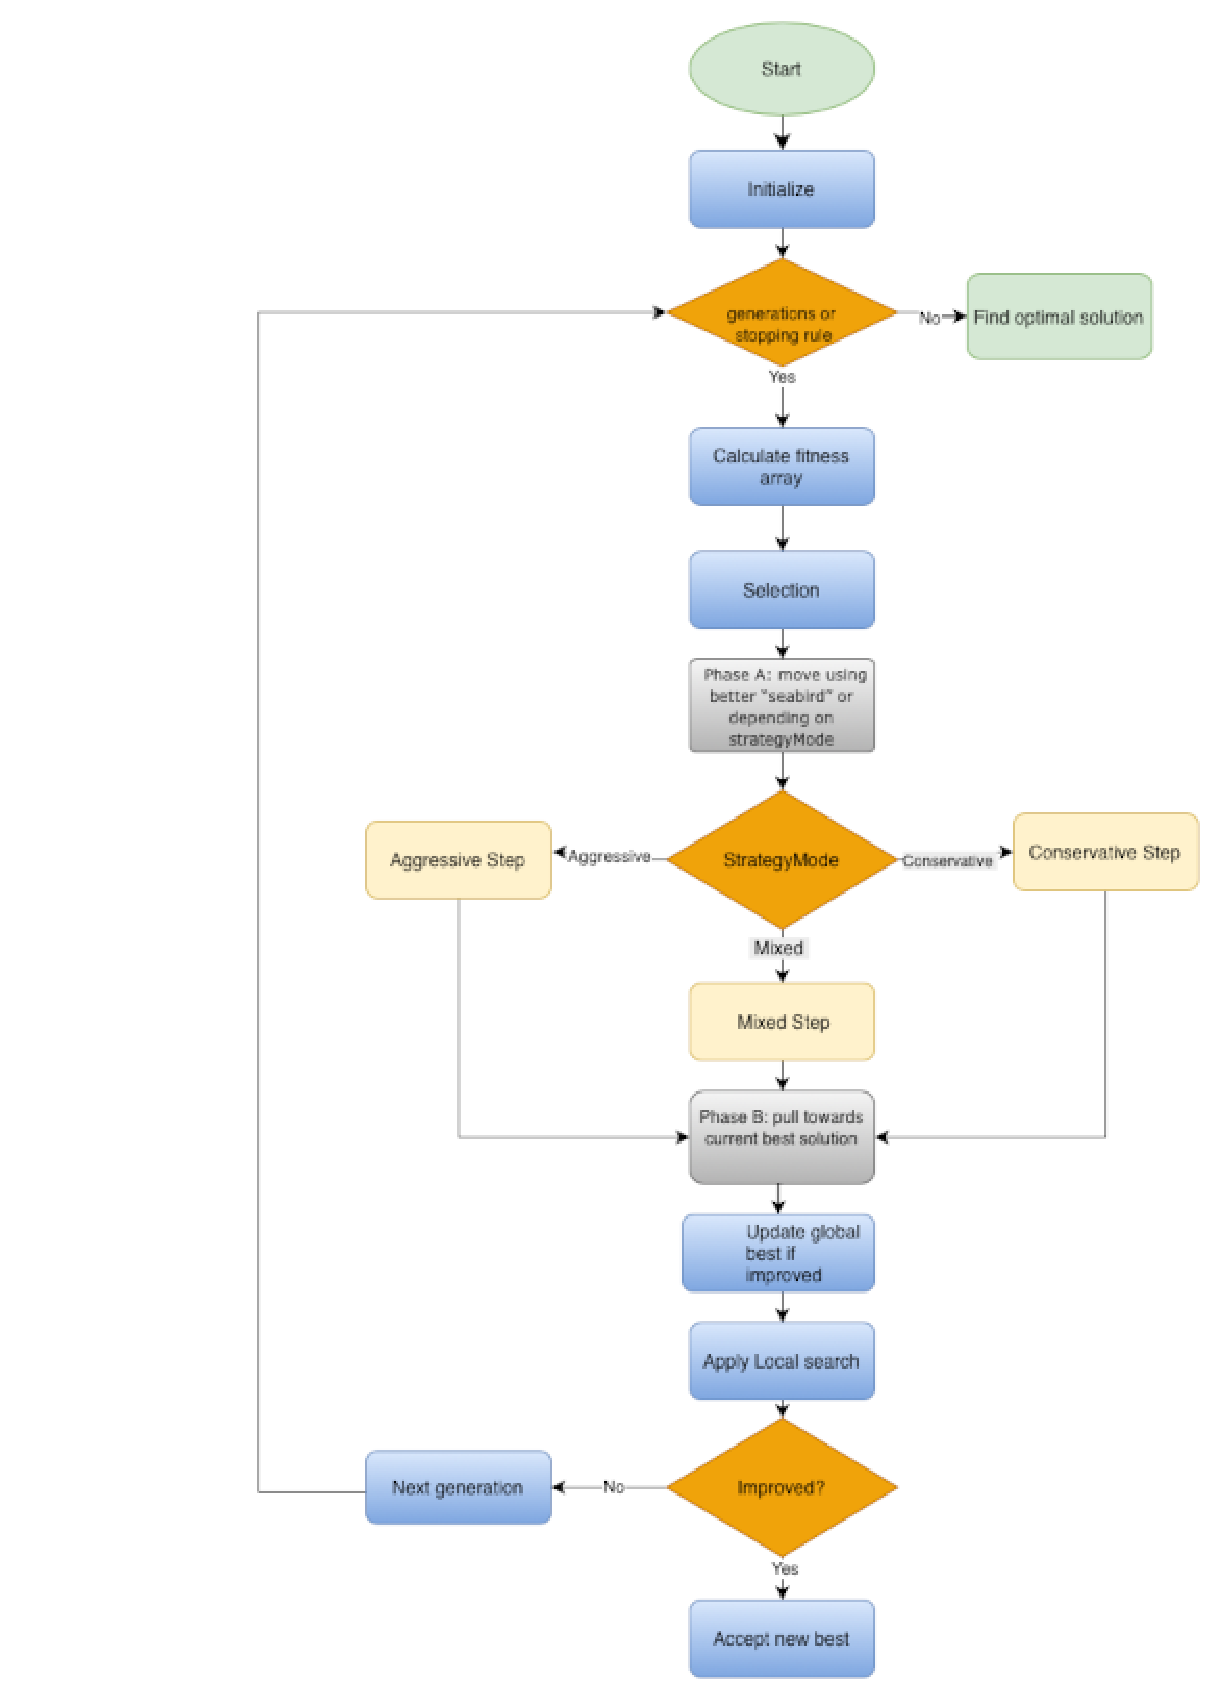
\includegraphics[scale=0.5]{mfo.eps}\caption{The steps of the proposed method \label{fig:Algorithm}}
\end{figure}


\subsection{The used termination rule\label{subsec:The-used-termination}}

The used termination rule is provided in the work of Charilogis and
Tsoulos \citep{stopping rule2} and it has the following steps:
\begin{itemize}
\item At every iteration $t$, the difference between the current best value
$f_{min}^{(t)}$ and the previous best value $f_{min}^{(t-1)}$ is
computed:
\end{itemize}
\begin{center}
\begin{equation}
\delta^{(t)}=\left|f_{\mbox{min}}^{(k)}-f_{\mbox{min}}^{(k-1)}\right|\label{eq:best}
\end{equation}
\par\end{center}
\begin{itemize}
\item The algorithm terminates when $\delta^{(t)}\le\epsilon$ for series
of predefined consecutive iterations $N_{k}$, where $\epsilon$ is
a small positive number, for example $10^{-6}$.
\end{itemize}

\subsection{Movement Strategies}

The proposed optimization algorithm employs three distinct movement
strategies that regulate the behavioral dynamics of seabirds during
the search for optimal solutions. Each strategy defines a different
balance between exploration of the search space and exploitation of
promising regions already identified.

The aggressive strategy is characterized by strong stochastic dynamics
and a tendency toward rapid discovery of new, potentially better regions
in the search space. Individuals are driven toward other, more successful
members of the population, performing large displacements that enhance
diversity and dispersion. This approach promotes exploration and enables
the algorithm to escape local optima. However, it also increases the
risk of generating infeasible or inefficient solutions if appropriate
boundary control mechanisms are not applied.

The conservative strategy focuses on exploitation of the best-known
solution, promoting smoother and more stable movements. Individuals
move gradually toward the current global best position with limited
randomness, aiming to refine the accuracy of their position over time.
This strategy reduces population diversity and enhances convergence.

The mixed strategy acts as an adaptive balance mechanism between the
two aforementioned approaches. At each iteration, the algorithm randomly
decides whether to apply the aggressive or conservative movement pattern,
allowing dynamic transitions between exploration and exploitation
phases. This flexibility enables the search process to adjust to the
evolving characteristics of the optimization landscape, preventing
premature convergence and maintaining adaptive search capability.

The integration of these three strategies ensures that the algorithm
maintains both exploratory power, essential for discovering new regions,
and exploitative stability, crucial for fine-tuning solutions. In
conclusion, their combined action enhances the robustness and efficiency
of the method.


\section{Results\label{sec:Results} }

This section begins with a description of the functions that will
be used in the experiments and then presents in detail the experiments
that were performed, in which the parameters available in the proposed
algorithm were studied, in order to study its reliability and adequacy. 

\subsection{Test Functions}

A variety of test functions were used in the conducted experiments\citep{testfunctions1,testfunctions2,testfunctions3,testfunctions4,testfunctions5,gkls}.
These functions are used in a series of research papers. The description
of each used test function is provided below. In all cases, the constant
$n$ defines the dimension of the objective function\@.
\begin{center}
{\tiny{}
\begin{table}
\centering{}{\tiny{}%
\begin{tabular}{|c|c|c|c|}
\hline 
{\tiny\textbf{NAME}} & {\tiny\textbf{FORMULA}} & {\tiny\textbf{DIM}} & {\tiny$G_{min}$}\tabularnewline
\hline 
\hline 
{\tiny\textbf{ACKLEY}} & \begin{cellvarwidth}[t]
\centering
{\tiny$f(x)=-a\exp\left(-b\sqrt{\frac{1}{n}\sum_{i=1}^{n}x_{i}^{2}}\right)-\exp\left(\frac{1}{n}\sum_{i=1}^{n}\cos\left(cx_{i}\right)\right)+a+\exp(1)$}{\tiny\par}

{\tiny$a=20.0,b=0.2$}
\end{cellvarwidth} & {\tiny 2} & {\tiny 4.440892099e-16}\tabularnewline
\hline 
{\tiny\textbf{BF1}} & {\tiny$f(x)=x_{1}^{2}+2x_{2}^{2}-\frac{3}{10}\cos\left(3\pi x_{1}\right)-\frac{4}{10}\cos\left(4\pi x_{2}\right)+\frac{7}{10}$} & {\tiny 2} & {\tiny 0}\tabularnewline
\hline 
{\tiny\textbf{BF2}} & {\tiny$f(x)=x_{1}^{2}+2x_{2}^{2}-\frac{3}{10}\cos\left(3\pi x_{1}\right)\cos\left(4\pi x_{2}\right)+\frac{3}{10}$} & {\tiny 2} & {\tiny 0}\tabularnewline
\hline 
{\tiny\textbf{BF3}} & {\tiny$f(x)=x_{1}^{2}+2x_{2}^{2}-\frac{3}{10}\cos\left(3\pi x_{1}+4\pi x_{2}\right)+\frac{3}{10}$} & {\tiny 2} & {\tiny 0}\tabularnewline
\hline 
{\tiny\textbf{BRANIN}} & \begin{cellvarwidth}[t]
\centering
{\tiny$f(x)=\left(x_{2}-\frac{5.1}{4\pi^{2}}x_{1}^{2}+\frac{5}{\pi}x_{1}-6\right)^{2}+10\left(1-\frac{1}{8\pi}\right)\cos(x_{1})+10$}{\tiny\par}

{\tiny$-5\le x_{1}\le10,\ 0\le x_{2}\le15$}
\end{cellvarwidth} & {\tiny 2} & {\tiny 0.3978873577}\tabularnewline
\hline 
{\tiny\textbf{CAMEL}} & {\tiny$f(x)=4x_{1}^{2}-2.1x_{1}^{4}+\frac{1}{3}x_{1}^{6}+x_{1}x_{2}-4x_{2}^{2}+4x_{2}^{4},\quad x\in[-5,5]^{2}$} & {\tiny 2} & {\tiny -1.031628453}\tabularnewline
\hline 
{\tiny\textbf{DIFFERENT POWERS}} & {\tiny$f(\mathbf{x})=\sqrt{\sum_{i=1}^{n}|x_{i}|^{2+4\frac{i-1}{n-1}}}$} & {\tiny n} & {\tiny 0}\tabularnewline
\hline 
{\tiny\textbf{DIFFPOWER}} & {\tiny$f(x)=\sum_{i=1}^{n}|x_{i}-y_{i}|^{p}$$\ \ n=2\ p=2,5,10$} & {\tiny n} & {\tiny 0}\tabularnewline
\hline 
{\tiny\textbf{DISCUS}} & {\tiny$f(x)=10^{6}x_{1}^{2}+\sum_{i=2}^{n}x_{i}^{2}$} & {\tiny n} & {\tiny 0}\tabularnewline
\hline 
{\tiny\textbf{EASOM}} & {\tiny$f(x)=-\cos\left(x_{1}\right)\cos\left(x_{2}\right)\exp\left(\left(x_{2}-\pi\right)^{2}-\left(x_{1}-\pi\right)^{2}\right)$} & {\tiny 2} & {\tiny -1}\tabularnewline
\hline 
{\tiny\textbf{ELLIPSOIDAL}} & {\tiny$f(x)=\sum_{i=1}^{n}\left(10^{6}\right)^{\frac{i-1}{n-1}}x_{i}^{2}$} & {\tiny n} & {\tiny 0}\tabularnewline
\hline 
{\tiny\textbf{EQUAL MAXIMA}} & {\tiny$f(x)=\sin^{6}(5\pi x)\cdot e^{-2\log(2)\cdot\left(\frac{x-0.1}{0.8}\right)^{2}}$} & {\tiny n} & {\tiny 0}\tabularnewline
\hline 
{\tiny\textbf{EXP}} & {\tiny$f(x)=-\exp\left(-0.5\sum_{i=1}^{n}x_{i}^{2}\right),\quad-1\le x_{i}\le1$} & {\tiny n} & {\tiny -1}\tabularnewline
\hline 
{\tiny\textbf{GKLS}} & {\tiny$f(x)=\mbox{Gkls}(x,n,w)$$\ \ n=2,3\ w=50,100$} & {\tiny n} & {\tiny -1}\tabularnewline
\hline 
{\tiny\textbf{GOLDSTAIN}} & \begin{cellvarwidth}[t]
\centering
{\tiny$f(x)=[1+(x_{1}+x_{2+1)})^{2}(19-14x_{1}+3x_{1}^{2}14x_{2}+6x_{1}x_{2}+3x_{2}^{2})]$}{\tiny\par}

{\tiny$[30+(2x_{1}-3x_{2})^{2}(18-32x_{1}+12x_{1}^{2}+48x_{2}-36x_{1}x_{2}+27x_{2}^{2})]$}
\end{cellvarwidth} & {\tiny 2} & {\tiny 3}\tabularnewline
\hline 
\begin{cellvarwidth}[t]
\centering
{\tiny\textbf{GRIEWANK}}{\tiny\par}

{\tiny\textbf{ROSENBROCK}}
\end{cellvarwidth} & {\tiny$f(\mathbf{x})=\underbrace{\left(\frac{\|\mathbf{x}\|^{2}}{4000}-\prod_{i=1}^{n}\cos\left(\frac{x_{i}}{\sqrt{i}}\right)+1\right)}_{\text{Griewank}}\cdot\underbrace{\left(\frac{1}{10}\sum_{i=1}^{n-1}\left[100(x_{i+1}-x_{i}^{2})^{2}+(1-x_{i})^{2}\right]\right)}_{\text{Rosenbrock}}$} & {\tiny n} & {\tiny 0}\tabularnewline
\hline 
{\tiny\textbf{GRIEWANK}} & {\tiny$f(x)=1+\frac{1}{200}\sum_{i=1}^{n}x_{i}^{2}-\prod_{i=1}^{n}\frac{\cos(x_{i})}{\sqrt{(i)}}$} & {\tiny n} & {\tiny 0}\tabularnewline
\hline 
{\tiny\textbf{HANSEN}} & {\tiny$f(x)=\sum_{i=1}^{5}i\cos\left[(i-1)x_{1}+i\right]\sum_{j=1}^{5}j\cos\left[(j+1)x_{2}+j\right]$} & {\tiny 2} & {\tiny -176.5417931}\tabularnewline
\hline 
{\tiny\textbf{HARTMAN3}} & {\tiny$f(x)=-\sum_{i=1}^{4}c_{i}\exp\left(-\sum_{j=1}^{3}a_{ij}\left(x_{j}-p_{ij}\right)^{2}\right)$} & {\tiny 3} & {\tiny -3.862782148}\tabularnewline
\hline 
{\tiny\textbf{HARTAMAN6}} & {\tiny$f(x)=-\sum_{i=1}^{4}c_{i}\exp\left(-\sum_{j=1}^{6}a_{ij}\left(x_{j}-p_{ij}\right)^{2}\right)$} & {\tiny 6} & {\tiny -3.22368011}\tabularnewline
\hline 
{\tiny\textbf{KATSUURA}} & {\tiny$f(\mathbf{x})=\frac{10}{n^{2}}\prod_{i=1}^{n}\left(1+i\sum_{k=1}^{32}\frac{|2^{k}x_{i}-\lfloor2^{k}x_{i}\rfloor|}{2^{k}}\right)^{\frac{10}{n^{1.2}}}-\frac{10}{n^{2}}+\frac{1}{Dn}\sum_{i=1}^{n}x_{i}^{2}$} & {\tiny n} & {\tiny 0}\tabularnewline
\hline 
{\tiny\textbf{MICHALEWICZ}} & {\tiny$f(\mathbf{x})=-\sum_{i=1}^{n}\sin(x_{i})\cdot\sin^{2m}\left(\frac{i\cdot x_{i}^{2}}{\pi}\right)$} & \begin{cellvarwidth}[t]
\centering
{\tiny 2,}{\tiny\par}

{\tiny 5,}{\tiny\par}

{\tiny 10}
\end{cellvarwidth} & \begin{cellvarwidth}[t]
\centering
{\tiny -1.8013}{\tiny\par}

{\tiny -4.6877}{\tiny\par}

{\tiny -9.6602}
\end{cellvarwidth}\tabularnewline
\hline 
{\tiny\textbf{POTENTIAL}} & {\tiny$V_{LJ}(r)=4\epsilon\left[\left(\frac{\sigma}{r}\right)^{12}-\left(\frac{\sigma}{r}\right)^{6}\right]$$\ \ n=9,15,21,30$} & \begin{cellvarwidth}[t]
\centering
{\tiny 5,}{\tiny\par}

{\tiny 6,}{\tiny\par}

{\tiny 10}
\end{cellvarwidth} & \begin{cellvarwidth}[t]
\centering
{\tiny -9.103852416}{\tiny\par}

{\tiny -12.71206226}{\tiny\par}

{\tiny -28.42253189}
\end{cellvarwidth}\tabularnewline
\hline 
{\tiny\textbf{RARSTIGIN2}} & {\tiny$f(x)=x_{1}^{2}+x_{2}^{2}-\cos(18x_{1})-\cos(18x_{2})$} & {\tiny 2} & {\tiny -2}\tabularnewline
\hline 
{\tiny\textbf{ROSENBROCK}} & {\tiny$f(x)=\sum_{i=1}^{n-1}\left(100\left(x_{i+1}-x_{i}^{2}\right)^{2}+\left(x_{i}-1\right)^{2}\right),\quad-30\le x_{i}\le30$} & {\tiny n} & {\tiny 0}\tabularnewline
\hline 
{\tiny\textbf{SHARP RIDGE}} & {\tiny$f(\mathbf{x})=x_{1}^{2}+\alpha\sum_{i=2}^{n}x_{i}^{2},\ a>1$} & {\tiny n} & {\tiny 0}\tabularnewline
\hline 
{\tiny\textbf{SHEKEL5}} & {\tiny$f(x)=-\sum_{i=1}^{5}\frac{1}{(x-a_{i})(x-a_{i})^{T}+c_{i}}$} & {\tiny 4} & {\tiny -10.10774912}\tabularnewline
\hline 
{\tiny\textbf{SHEKEL7}} & {\tiny$f(x)=-\sum_{i=1}^{7}\frac{1}{(x-a_{i})(x-a_{i})^{T}+c_{i}}$} & {\tiny 4} & {\tiny -10.342377774}\tabularnewline
\hline 
{\tiny\textbf{SHEKEL10}} & {\tiny$f(x)=-\sum_{i=1}^{10}\frac{1}{(x-a_{i})(x-a_{i})^{T}+c_{i}}$} & {\tiny 4} & {\tiny -10.53640982}\tabularnewline
\hline 
{\tiny\textbf{SINUSOIDAL}} & {\tiny$f(x)=-\left(2.5\prod_{i=1}^{n}\sin\left(x_{i}-z\right)+\prod_{i=1}^{n}\sin\left(5\left(x_{i}-z\right)\right)\right),\quad0\le x_{i}\le\pi$} & {\tiny n} & {\tiny -3.5}\tabularnewline
\hline 
{\tiny\textbf{SPHERE}} & {\tiny$f(\mathbf{x})=\sum_{i=1}^{n}x_{i}^{2}$} & {\tiny n} & {\tiny 0}\tabularnewline
\hline 
{\tiny\textbf{STEP ELLIPSOIDAL}} & {\tiny$f(\mathbf{x})=\sum_{i=1}^{n}\left\lfloor x_{i}+0.5\right\rfloor ^{2}+\alpha\sum_{i=1}^{n}\left(10^{6}\cdot\frac{i-1}{n-1}\right)x_{i}^{2},\ a=1$} & {\tiny n} & {\tiny 0}\tabularnewline
\hline 
{\tiny\textbf{TEST2N}} & {\tiny$f(x)=\frac{1}{2}\sum_{i=1}^{n}x_{i}^{4}-16x_{i}^{2}+5x_{i}$} & \begin{cellvarwidth}[t]
\centering
{\tiny 4,}{\tiny\par}

{\tiny 5}
\end{cellvarwidth} & \begin{cellvarwidth}[t]
\centering
{\tiny -156.6646628}{\tiny\par}

{\tiny -195.8308285}
\end{cellvarwidth}\tabularnewline
\hline 
{\tiny\textbf{TEST30N}} & \begin{cellvarwidth}[t]
\centering
{\tiny$f(x)=\frac{1}{10}\sin^{2}\left(3\pi x_{1}\right)\sum_{i=2}^{n-1}\left(\left(x_{i}-1\right)^{2}\left(1+\sin^{2}\left(3\pi x_{i+1}\right)\right)\right)+$}{\tiny\par}

{\tiny$+\left(x_{n}-1\right)^{2}\left(1+\sin^{2}\left(2\pi x_{n}\right)\right)$}
\end{cellvarwidth} & {\tiny n} & {\tiny 0}\tabularnewline
\hline 
{\tiny\textbf{ZAKHAROV}} & {\tiny$f(\mathbf{x})=\sum_{i=1}^{n}x_{i}^{2}+\left(\sum_{i=1}^{n}\frac{i}{2}x_{i}\right)^{2}+\left(\sum_{i=1}^{n}\frac{i}{2}x_{i}\right)^{4}$} & {\tiny n} & {\tiny 0}\tabularnewline
\hline 
\end{tabular}}
\end{table}
}{\tiny\par}
\par\end{center}

\subsection{Experimental results }

A series of experiments was carried out for the previously mentioned
functions and these experiments were executed on an AMD RYZEN 5950X
with 128GB RAM. The operating system of the running machine was Debian
Linux. Each experiment was conducted 30 times, with different random
numbers each time, and the averages were recorded. The software used
in the experiments was coded in ANSI C++ using the freely available
optimization environment of OPTIMUS, which can be downloaded from\textbf{
}\url{https://github.com/itsoulos/OPTIMUS}. The values for the experimental
parameters used in the proposed method are outlined in Table \ref{tab:expSettings}. 

\begin{table}[H]
\caption{The values of the parameters of the proposed method.\label{tab:expSettings}}

\centering{}%
\begin{tabular}{|c|c|c|}
\hline 
PARAMETER & MEANING & VALUE\tabularnewline
\hline 
\hline 
N & Number of agents & 200\tabularnewline
\hline 
$G_{max}$ & Maximum number of allowed iterations & 200\tabularnewline
\hline 
$p_{l}$ & Local search rate & 0.05\tabularnewline
\hline 
T & Number of mfo iterations & 2\tabularnewline
\hline 
\end{tabular}
\end{table}
In the following tables that depict the experimental results, the
numbers in cells stand for the average function calls, as measured
on 30 independent runs. The numbers in parentheses denote the fraction
of the executions where the method discovered successfully the global
minimum. If this number is not present, then the method managed to
locate the global minimum in every run ( 100\% success).

\subsection{The proposed method in comparison with others}

The comparison of results for nine optimization methods (PROPOSED,
GENETIC\citep{genetic3}, WOA\citep{key-22}, MEWOA\citep{key-21},
DE\citep{diffe1}, IPSO\citep{key-23}, AOA\citep{key-4}, SAO\citep{key-5}
and ACO\citep{aco1}) is based on a diverse set of benchmark functions.
The evaluation focused on two key performance indicators: the total
number of objective function evaluations and the corresponding success
rates, as shown in Table 2.

The analysis of the total function evaluations reveals substantial
differences among the tested algorithms. The GENETIC algorithm required
316,189 evaluations, while WOA recorded the highest computational
cost with 923,113 evaluations. The MEWOA, DE, IPSO, AOA, SAO, and
ACO methods required 489,691, 326,083, 314,060, 540,139, 305,505,
and 260,753 evaluations, respectively. In contrast, the PROPOSED algorithm
achieved the lowest total number of function evaluations, requiring
only 204,488 calls in total, demonstrating exceptional computational
efficiency.

This superiority was true for almost all reference functions. For
example, on the Ackley function, the PROPOSED method reached convergence
in only 4971 evaluations, while GENETIC and WOA required 5811 and
24,766 evaluations, respectively. Similarly, for the Branin function,
the PROPOSED algorithm required 2397 evaluations, much fewer than
GENETIC's 2648 and AOA's 4777 for this function.

In addition to the reduced computational cost, the PROPOSED algorithm
maintained a 100\% success rate for most benchmark functions, confirming
its reliability. Also, the DE, IPSO and SAO algorithms also produced
satisfactory results, but with higher computational cost. In contrast,
the ACO algorithm presented lower consistency, with success rates
below unity (e.g., 0.57 for BF1 and 0.70 for BF2).

The results show that the PROPOSED algorithm is very efficient and
reliable. It manages to give equally good or even better results than
other known algorithms, but with much fewer calculations. 

{\tiny{}
\begin{table}
{\tiny\caption{Experimental results using different optimization methods. Numbers
in cells represent sum function calls.}
}{\tiny\par}
\raggedright{}{\tiny{}%
\begin{tabular}{|c|c|c|c|c|c|c|c|c|c|}
\hline 
{\tiny\textbf{FUNCTION}} & {\tiny\textbf{PROPOSED}} & {\tiny\textbf{GENETIC}} & {\tiny\textbf{WOA}} & {\tiny\textbf{MEWOA}} & {\tiny\textbf{DE}} & {\tiny\textbf{IPSO}} & {\tiny\textbf{AOA}} & {\tiny\textbf{SAO}} & {\tiny\textbf{ACO}}\tabularnewline
\hline 
\hline 
{\tiny ACKLEY} & {\tiny 4971} & {\tiny 5811} & {\tiny 24766} & {\tiny 15257} & {\tiny 6425} & {\tiny 7355} & {\tiny 9590} & {\tiny 5904} & {\tiny 6112}\tabularnewline
\hline 
{\tiny BF1} & {\tiny 3449} & {\tiny 4279} & {\tiny 9924} & {\tiny 8423} & {\tiny 4272} & {\tiny 4121} & {\tiny 8356} & {\tiny 4694} & {\tiny 4120(0.57)}\tabularnewline
\hline 
{\tiny BF2} & {\tiny 3255} & {\tiny 3903} & {\tiny 9597} & {\tiny 7982} & {\tiny 3863} & {\tiny 3767} & {\tiny 6987} & {\tiny 4166} & {\tiny 3613(0.70)}\tabularnewline
\hline 
{\tiny BF3} & {\tiny 3028} & {\tiny 3494} & {\tiny 20117} & {\tiny 7087} & {\tiny 3475} & {\tiny 3305} & {\tiny 7029} & {\tiny 3706} & {\tiny 3563(0.77)}\tabularnewline
\hline 
{\tiny BRANIN} & {\tiny 2397} & {\tiny 2648} & {\tiny 5939} & {\tiny 4170} & {\tiny 2543} & {\tiny 2522} & {\tiny 4777} & {\tiny 2583} & {\tiny 2814}\tabularnewline
\hline 
{\tiny CAMEL} & {\tiny 2757} & {\tiny 3104} & {\tiny 5917} & {\tiny 5854} & {\tiny 3054} & {\tiny 2942} & {\tiny 5050} & {\tiny 3089} & {\tiny 2421}\tabularnewline
\hline 
\begin{cellvarwidth}[t]
\centering
{\tiny DIFFERENT}\\
{\tiny POWERS10}
\end{cellvarwidth} & {\tiny 6651} & {\tiny 10954} & {\tiny 23650} & {\tiny 16588} & {\tiny 10542} & {\tiny 9807} & {\tiny 27533} & {\tiny 11234} & {\tiny 10471}\tabularnewline
\hline 
{\tiny DIFFPOWER2} & {\tiny 5614} & {\tiny 9053} & {\tiny 13476} & {\tiny 14248} & {\tiny 8510} & {\tiny 8121} & {\tiny 14367} & {\tiny 9139} & {\tiny 10540}\tabularnewline
\hline 
{\tiny DIFFPOWER5} & {\tiny 13836} & {\tiny 24466} & {\tiny 51816} & {\tiny 40313} & {\tiny 25515} & {\tiny 27348} & {\tiny 58890} & {\tiny 27918} & {\tiny 32583}\tabularnewline
\hline 
{\tiny DIFFPOWER10} & {\tiny 19486} & {\tiny 37664} & {\tiny 73782} & {\tiny 56980} & {\tiny 40402} & {\tiny 34923} & {\tiny 74297} & {\tiny 39429} & {\tiny 16664}\tabularnewline
\hline 
{\tiny DISCUS10} & {\tiny 2185} & {\tiny 2711} & {\tiny 6476} & {\tiny 4084} & {\tiny 2663} & {\tiny 2540} & {\tiny 6302} & {\tiny 2716} & {\tiny 2010}\tabularnewline
\hline 
{\tiny EASOM} & {\tiny 2033} & {\tiny 2062} & {\tiny 3153} & {\tiny 3194} & {\tiny 1953} & {\tiny 1998} & {\tiny 2691} & {\tiny 2167} & {\tiny 1995}\tabularnewline
\hline 
{\tiny ELLIPSOIDAL10} & {\tiny 2479} & {\tiny 3309} & {\tiny 8979} & {\tiny 5057} & {\tiny 3339} & {\tiny 3540} & {\tiny 6308} & {\tiny 2507} & {\tiny 2146}\tabularnewline
\hline 
{\tiny EQUALMAXIMA10} & {\tiny 8968} & {\tiny 16399} & {\tiny 63542} & {\tiny 26257} & {\tiny 17891} & {\tiny 17231} & {\tiny 20536} & {\tiny 17014} & {\tiny 18343}\tabularnewline
\hline 
{\tiny EXPONENTIAL10} & {\tiny 2768} & {\tiny 3854} & {\tiny 8408} & {\tiny 6224} & {\tiny 3928} & {\tiny 3298} & {\tiny 6216} & {\tiny 3052} & {\tiny 3941}\tabularnewline
\hline 
{\tiny GKLS250} & {\tiny 2701} & {\tiny 2579} & {\tiny 4978} & {\tiny 4481} & {\tiny 2412} & {\tiny 2580} & {\tiny 3220} & {\tiny 1789} & {\tiny 2238}\tabularnewline
\hline 
{\tiny GKLS350} & {\tiny 3054} & {\tiny 3076} & {\tiny 7226(0.96)} & {\tiny 4117} & {\tiny 2860} & {\tiny 3016} & {\tiny 3314} & {\tiny 1634(0.86)} & {\tiny 2110(0.90)}\tabularnewline
\hline 
{\tiny GOLDSTEIN} & {\tiny 3195} & {\tiny 3802} & {\tiny 9016} & {\tiny 6598} & {\tiny 3736} & {\tiny 3856} & {\tiny 6508} & {\tiny 3522} & {\tiny 4239}\tabularnewline
\hline 
{\tiny GRIEWANK2} & {\tiny 4289(0.80)} & {\tiny 4313(0.73)} & {\tiny 7948(0.87)} & {\tiny 6613(0.96)} & {\tiny 4689(0.80)} & {\tiny 4516} & {\tiny 6339(0.73)} & {\tiny 4881(0.73)} & {\tiny 3624(0.43)}\tabularnewline
\hline 
{\tiny GRIEWANK10} & {\tiny 5374} & {\tiny 8381} & {\tiny 51143} & {\tiny 14380} & {\tiny 8888} & {\tiny 8087} & {\tiny 16979} & {\tiny 8788} & {\tiny 5679}\tabularnewline
\hline 
\begin{cellvarwidth}[t]
\centering
{\tiny GRIEWANK}\\
{\tiny ROSENBROCK10}
\end{cellvarwidth} & {\tiny 5505} & {\tiny 9576} & {\tiny 16592} & {\tiny 13856} & {\tiny 9923} & {\tiny 7675} & {\tiny 17936} & {\tiny 9157} & {\tiny 3694}\tabularnewline
\hline 
{\tiny HANSEN} & {\tiny 3531} & {\tiny 3345} & {\tiny 10498} & {\tiny 5072} & {\tiny 3189} & {\tiny 3546} & {\tiny 4166} & {\tiny 3245} & {\tiny 3042(0.70)}\tabularnewline
\hline 
{\tiny HARTMAN3} & {\tiny 2633} & {\tiny 3142} & {\tiny 8440} & {\tiny 5095} & {\tiny 3177} & {\tiny 3103} & {\tiny 4034} & {\tiny 2539} & {\tiny 3297}\tabularnewline
\hline 
{\tiny HARTMAN6} & {\tiny 2874} & {\tiny 3941} & {\tiny 22615} & {\tiny 6214} & {\tiny 3870} & {\tiny 3688} & {\tiny 5468} & {\tiny 3019} & {\tiny 3949(0.77)}\tabularnewline
\hline 
{\tiny KATSUURA10} & {\tiny 8648(0.03)} & {\tiny 19539(0.03)} & {\tiny 61156(0.33)} & {\tiny 25791(0.03)} & {\tiny 22199(0.03)} & {\tiny 16452(0.03)} & {\tiny 24172(0.03)} & {\tiny 18650(0.03)} & {\tiny 24341(0.03)}\tabularnewline
\hline 
{\tiny MICHALEWICZ4} & {\tiny 3757(0.63)} & {\tiny 5906(0.90)} & {\tiny 14045(0.87)} & {\tiny 7419(0.97)} & {\tiny 5186(0.97)} & {\tiny 4583(0.93)} & {\tiny 5746(0.93} & {\tiny 4176(0.80)} & {\tiny 4213(0.17)}\tabularnewline
\hline 
{\tiny POTENTIAL5} & {\tiny 4944} & {\tiny 8166} & {\tiny 39455} & {\tiny 12218} & {\tiny 8525} & {\tiny 10128} & {\tiny 10883} & {\tiny 7879} & {\tiny 7456}\tabularnewline
\hline 
{\tiny POTENTIAL6} & {\tiny 5887(0.37)} & {\tiny 12034(0.80)} & {\tiny 46466(0.77)} & {\tiny 13728(0.77)} & {\tiny 12073(0.73)} & {\tiny 13873(0.47)} & {\tiny 11948(0.67)} & {\tiny 9564(0.70)} & {\tiny 8212(0.13)}\tabularnewline
\hline 
{\tiny POTENTIAL10} & {\tiny 8599(0.93)} & {\tiny 15417} & {\tiny 59487} & {\tiny 23210} & {\tiny 16382} & {\tiny 21690(0.97)} & {\tiny 18199(0.96)} & {\tiny 14463} & {\tiny 9235(0.27)}\tabularnewline
\hline 
{\tiny RASTRIGIN} & {\tiny 3639} & {\tiny 3840(0.93)} & {\tiny 8116} & {\tiny 6127} & {\tiny 4287} & {\tiny 3956} & {\tiny 5052} & {\tiny 2813(0.93)} & {\tiny 2676(0.33)}\tabularnewline
\hline 
{\tiny ROSENBROCK8} & {\tiny 4964} & {\tiny 8085} & {\tiny 14094} & {\tiny 12282} & {\tiny 8245} & {\tiny 7843} & {\tiny 16423} & {\tiny 8448} & {\tiny 2893}\tabularnewline
\hline 
{\tiny ROSENBROCK16} & {\tiny 6467} & {\tiny 11469} & {\tiny 23544} & {\tiny 17851} & {\tiny 11999} & {\tiny 11450} & {\tiny 25092} & {\tiny 12016} & {\tiny 3604}\tabularnewline
\hline 
{\tiny SHARPRIDGE10} & {\tiny 6006} & {\tiny 10297} & {\tiny 18391} & {\tiny 15280} & {\tiny 10924} & {\tiny 10481} & {\tiny 22452} & {\tiny 10013} & {\tiny 3594}\tabularnewline
\hline 
{\tiny SHEKEL5} & {\tiny 3230} & {\tiny 4540} & {\tiny 17010} & {\tiny 6551} & {\tiny 4361} & {\tiny 3986} & {\tiny 7615} & {\tiny 4271} & {\tiny 4492(0.63)}\tabularnewline
\hline 
{\tiny SHEKEL7} & {\tiny 3212} & {\tiny 4517} & {\tiny 17873} & {\tiny 6985} & {\tiny 4310} & {\tiny 4009} & {\tiny 7491} & {\tiny 4245} & {\tiny 4719(0.67)}\tabularnewline
\hline 
{\tiny SHEKEL10} & {\tiny 3168} & {\tiny 4266} & {\tiny 15524} & {\tiny 6750} & {\tiny 4217} & {\tiny 4010} & {\tiny 7074} & {\tiny 4111} & {\tiny 4442(0.47)}\tabularnewline
\hline 
{\tiny SPHERE10} & {\tiny 1660} & {\tiny 1706} & {\tiny 6389} & {\tiny 2927} & {\tiny 1653} & {\tiny 1636} & {\tiny 5128} & {\tiny 906} & {\tiny 1843}\tabularnewline
\hline 
\begin{cellvarwidth}[t]
\centering
{\tiny STEPE}\\
{\tiny LLIPSOIDAL4}
\end{cellvarwidth} & {\tiny 3018} & {\tiny 2842(0.83)} & {\tiny 2129} & {\tiny 2237(0.93)} & {\tiny 2385(0.73)} & {\tiny 1879} & {\tiny 2701(0.43)} & {\tiny 1262(0.07)} & {\tiny 1583(0.10)}\tabularnewline
\hline 
{\tiny SINUSOIDAL8} & {\tiny 3272} & {\tiny 4572} & {\tiny 20782} & {\tiny 7032} & {\tiny 4519} & {\tiny 3995} & {\tiny 7249} & {\tiny 3901} & {\tiny 4023(0.83)}\tabularnewline
\hline 
{\tiny SINUSOIDAL16} & {\tiny 4454(0.93)} & {\tiny 6588} & {\tiny 34409} & {\tiny 9368} & {\tiny 7349} & {\tiny 4697} & {\tiny 10405} & {\tiny 6491} & {\tiny 4669(0.63)}\tabularnewline
\hline 
{\tiny TEST2N4} & {\tiny 3236} & {\tiny 3878} & {\tiny 12279} & {\tiny 6019} & {\tiny 3699} & {\tiny 3611} & {\tiny 5765} & {\tiny 3251} & {\tiny 3504(0.56)}\tabularnewline
\hline 
{\tiny TEST2N5} & {\tiny 3639(0.97)} & {\tiny 4109(0.86)} & {\tiny 15351(0.83)} & {\tiny 6178} & {\tiny 4248(0.96)} & {\tiny 3977(0.93)} & {\tiny 6647(0.93)} & {\tiny 3569(0.97)} & {\tiny 3718(0.30)}\tabularnewline
\hline 
{\tiny TEST30N10} & {\tiny 3134} & {\tiny 5238} & {\tiny 16970} & {\tiny 8809} & {\tiny 5206} & {\tiny 6055} & {\tiny 7915} & {\tiny 4915} & {\tiny 6203}\tabularnewline
\hline 
{\tiny ZAKHAROV10} & {\tiny 2521} & {\tiny 3314} & {\tiny 11645} & {\tiny 4785} & {\tiny 3197} & {\tiny 2864} & {\tiny 5289} & {\tiny 2669} & {\tiny 2125}\tabularnewline
\hline 
{\tiny\textbf{SUM}} & {\tiny\textbf{204488(0.95)}} & {\tiny\textbf{316189(0.96)}} & {\tiny\textbf{923113(0.97)}} & {\tiny\textbf{489691(0.97)}} & {\tiny\textbf{326083(0.96)}} & {\tiny\textbf{314060(0.96)}} & {\tiny\textbf{540139(0.95)}} & {\tiny\textbf{305505(0.93)}} & {\tiny\textbf{260753(0.77)}}\tabularnewline
\hline 
\end{tabular}}{\tiny\par}
\end{table}
}{\tiny\par}

\begin{figure}
\includegraphics[scale=0.25]{figure2}

\caption{A statistical comparison of the proposed with other optimization methods}
\end{figure}

Figure 2 summarizes the pairwise significance between the PROPOSED
method and the baseline optimizers. Using the conventional star notation
(ns: p \textgreater{} 0.05, {*}: p \textless{} 0.05, {*}{*}: p \textless{}
0.01, {*}{*}{*}: p \textless{} 0.001, {*}{*}{*}{*}: p \textless{}
0.0001), all comparisons except ACO reach {*}{*}{*}{*}, indicating
very-extremely significant differences. Specifically, PROPOSED differs
from GENETIC, WOA, MEWOA, DE, IPSO, AOA and SAO at p \textless{} 0.0001,
whereas the comparison with ACO is not statistically significant (p
\textgreater{} 0.05). In conjunction with the reported performance
metrics, these results indicate that the advantage of PROPOSED over
most baselines is highly unlikely to be due to random variation.

\subsection{Comparative analysis of different strategic variations}

To further evaluate the internal adaptability of the proposed optimization
framework, three distinct strategic configurations: Aggressive, Conservative,
and Mixed were examined across a comprehensive set of benchmark functions.
The total number of objective function evaluations recorded for each
configuration was 204,488 for the aggressive strategy, 212,680 for
the conservative strategy, and 209,767 for the mixed strategy. Among
these, the aggressive configuration demonstrated the lowest computational
demand, indicating faster convergence behavior.

For example, the aggressive strategy in the Easom benchmark function
required 2033 evaluations and Potential5 required 4944 evaluations.
While in the conservative strategy Easom required 2178 evaluations
and Potential5 required 5,108 evaluations. On the other hand, in the
mixed strategy it required 2100 and 4914 evaluations in the corresponding
functions.

In terms of reliability, all three configurations demonstrated excellent
success rates, maintaining near-perfect consistency across most benchmark
functions. Specifically, the success rates were 95\% for the aggressive
strategy, 93\% for the conservative strategy, and 94\% for the mixed
configuration. The algorithm’s stable performance highlights its robustness,
as it stays reliable under different search strategies. Minor differences
mainly affect speed and computational effort.

Overall, the results show that the proposed framework is flexible
and adaptable, allowing its settings to adjust to different problems.
The Conservative version offers a good balance between accuracy and
speed, the Aggressive one works best on complex problems by avoiding
early convergence, and the Mixed approach provides a stable middle
ground. This adaptability makes the framework suitable for many optimization
tasks.

\begin{table}
\caption{Experiments using different strategy for the proposed method.}

\centering{}%
\begin{tabular}{|c|c|c|c|}
\hline 
\textbf{FUNCTION} & \textbf{AGGRESSIVE} & \textbf{CONSERVATIVE} & \textbf{MIXED}\tabularnewline
\hline 
\hline 
ACKLEY & 4971 & 4749 & 4881\tabularnewline
\hline 
BF1 & 3449 & 3541 & 3520\tabularnewline
\hline 
BF2 & 3255 & 3355 & 3291\tabularnewline
\hline 
BF3 & 3028 & 3090 & 3076\tabularnewline
\hline 
BRANIN & 2397 & 2548 & 2460\tabularnewline
\hline 
CAMEL & 2757 & 2854 & 2815\tabularnewline
\hline 
DIFFERENTPOWERS10 & 6651 & 6978 & 6803\tabularnewline
\hline 
DIFFPOWER2 & 5614 & 5451 & 5792\tabularnewline
\hline 
DIFFPOWER5 & 13836 & 13301 & 14807\tabularnewline
\hline 
DIFFPOWER10 & 19486 & 19332 & 19118\tabularnewline
\hline 
DISCUS10 & 2185 & 2424 & 2274\tabularnewline
\hline 
EASOM & 2033 & 2178 & 2100\tabularnewline
\hline 
ELLIPSOIDAL10 & 2479 & 2717 & 2566\tabularnewline
\hline 
EQUALMAXIMA10 & 8968 & 9069 & 8717\tabularnewline
\hline 
EXPONENTIAL10 & 2768 & 3065 & 2930\tabularnewline
\hline 
GKLS250 & 2701 & 2833 & 2769\tabularnewline
\hline 
GKLS350 & 3054 & 3583 & 3260\tabularnewline
\hline 
GOLDSTEIN & 3195 & 3243 & 3244\tabularnewline
\hline 
GRIEWANK2 & 4289(0.80) & 4319(0.67) & 4407(0.73)\tabularnewline
\hline 
GRIEWANK10 & 5374 & 5546 & 5249(0.97)\tabularnewline
\hline 
GRIEWANKROSENBROCK10 & 5505 & 5957 & 5806\tabularnewline
\hline 
HANSEN & 3531 & 3557(0.80) & 3288(0.93)\tabularnewline
\hline 
HARTMAN3 & 2633 & 2850 & 2755\tabularnewline
\hline 
HARTMAN6 & 2874 & 3182 & 2971\tabularnewline
\hline 
KATSUURA10 & 8648(0.03) & 9366(0.03) & 9109(0.03)\tabularnewline
\hline 
MICHALEWICZ4 & 3757(0.63) & 4099(0.60) & 4404(0.60)\tabularnewline
\hline 
POTENTIAL5 & 4944 & 5108 & 4914\tabularnewline
\hline 
POTENTIAL6 & 5887(0.37) & 6215(0.50) & 6451(0.56)\tabularnewline
\hline 
POTENTIAL10 & 8599(0.93) & 8745(0.93) & 8305(0.93)\tabularnewline
\hline 
RASTRIGIN & 3639 & 3660(0.93) & 3848\tabularnewline
\hline 
ROSENBROCK8 & 4964 & 5256 & 5137\tabularnewline
\hline 
ROSENBROCK16 & 6467 & 6929 & 6837\tabularnewline
\hline 
SHARPRIDGE10 & 6006 & 6287 & 6024\tabularnewline
\hline 
SHEKEL5 & 3230 & 3436 & 3317\tabularnewline
\hline 
SHEKEL7 & 3212 & 3405 & 3288\tabularnewline
\hline 
SHEKEL10 & 3168 & 3360 & 3270\tabularnewline
\hline 
SPHERE10 & 1660 & 1927 & 1791\tabularnewline
\hline 
STEPELLIPSOIDAL4 & 3018 & 3435(0.93) & 3245\tabularnewline
\hline 
SINUSOIDAL8 & 3272 & 3665 & 3499\tabularnewline
\hline 
SINUSOIDAL16 & 4454(0.93) & 4561(0.93) & 4576(0.93)\tabularnewline
\hline 
TEST2N4 & 3236 & 3434(0.93) & 3371(0.97)\tabularnewline
\hline 
TEST2N5 & 3639(0.97) & 3731(0.80) & 3511(0.77)\tabularnewline
\hline 
TEST30N10 & 3134 & 3590 & 3380\tabularnewline
\hline 
ZAKHAROV10 & 2521 & 2749 & 2591\tabularnewline
\hline 
\textbf{SUM} & \textbf{204488(0.95)} & \textbf{212680(0.93)} & \textbf{209767(0.94)}\tabularnewline
\hline 
\end{tabular}
\end{table}

\begin{figure}
\includegraphics[scale=0.25]{figure3}

\caption{A statistical comparison of the proposed method with different movement
strategies}

\end{figure}

In Figure 3 we report pairwise significance for the exploration-exploitation
control modes of the proposed optimizer. AGGRESSIVE vs CONSERVATIVE
reaches {*}{*}{*}{*} (p \textless{} 0.0001), indicating a very-extremely
significant difference. CONSERVATIVE vs MIXED is {*}{*} (p \textless{}
0.01), showing a highly significant separation. MIXED vs AGGRESSIVE
is {*}{*}{*} (p \textless{} 0.001), reflecting an extremely significant
but comparatively smaller gap. Overall, the regimes induce materially
different behaviors, with MIXED lying closer to AGGRESSIVE than to
CONSERVATIVE.

\subsection{Impact of Population Size on Algorithmic Performance}

To assess the influence of population size on convergence behavior
and computational efficiency, both the proposed optimization algorithm
and the Genetic Algorithm (GA) were evaluated under four different
population configurations: 50, 100, 200, and 500. The experiments
were conducted using a representative suite of benchmark functions.

In a population size of 50 individuals, both algorithms demonstrated
rapid convergence with low computational cost. The proposed algorithm
required only 1983 evaluations for the Ackley function, while BF1
required 1075 and BF2 required 983. The Genetic Algorithm converged
after 2148 evaluations for Ackley, while 1258 for BF1 and 1105 for
BF2. Despite their computational efficiency, both methods showed a
slight decline in success rate in certain benchmark functions due
to the limited population diversity. For example, the proposed algorithm
achieved success rates around 0.90 for BF2 and BF3, while the GA achieved
97\% for Ackley and 30\% for Griewank2. 

When the population size was increased to 100, both algorithms reached
their most balanced performance. The proposed algorithm achieved a
100\% success rate on almost all test functions with 3053 evaluations
for Ackley, 1862 for BF1, 1734 evaluations for BF2 and 1211 for Branin.
The Genetic Algorithm achieved comparable results, also maintaining
a 100\% success rate, with 3331 evaluations for Ackley, 2287 for BF1,
and 1353 for Branin. This configuration provided sufficient population
diversity for effective exploration without incurring significant
computational overhead. As a result, a medium-sized population offered
the optimal trade-off between exploration and exploitation, ensuring
both robustness and computational efficiency. 

Further increasing the population to 200 led to a significant increase
in computational cost for both algorithms. The proposed algorithm
required 4971 evaluations for Ackley while 3449 evaluations for BF1
and 3255 for BF2. The GA reached 5811 evaluations for Ackley and 3494
for BF3. Although the success rate slightly improved, the additional
computational effort did not yield proportional benefits in optimization
performance. 

When the population size was further increased to 500, this pattern
became even more apparent. The proposed algorithm required up to 10,690
evaluations for Ackley while 8346 for the BF1 function and 7825 for
the BF2 function. The GA needed 13,664 evaluations for Ackley, 10,866
for BF1, and 6716 for Branin. While both algorithms maintained high
success rates, the computational effort increased drastically, indicating
a prolonged and redundant exploratory phase that hindered convergence
speed and overall efficiency. 

The comparative analysis reveals a consistent trend for both algorithms:
population size has a direct and significant impact on convergence
dynamics and computational efficiency. Small populations favor faster
convergence but risk premature stagnation due to limited diversity.
Very large populations improve reliability but impose excessive computational
cost. Medium-sized populations achieve the best balance between speed,
accuracy, and robustness.

Overall, the proposed algorithm consistently outperformed the Genetic
Algorithm at all population levels, requiring fewer evaluations to
reach convergence while maintaining equal or higher success rates.
This improvement is attributed to its adaptive parameter control and
dynamic balance between local and global search, which enhance convergence
efficiency without compromising precision.

In summary, population size plays a crucial role in determining the
optimization efficiency of both algorithms. For practical applications,
a moderate population configuration ensures optimal performance, achieving
rapid, accurate, and stable convergence with minimal computational
overhead.
\begin{center}
{\tiny{}
\begin{table}
\begin{raggedright}
{\tiny{}%
\begin{tabular}{|c|c|c|c|c|c|c|c|c|}
\hline 
{\tiny\textbf{FUNCTION}} & {\tiny\textbf{N=50}} & {\tiny\textbf{GA(N=50)}} & {\tiny\textbf{N=100}} & {\tiny\textbf{GA(N=100)}} & {\tiny\textbf{N=200}} & {\tiny\textbf{GA(N=200)}} & {\tiny\textbf{N=500}} & {\tiny\textbf{GA(N=500)}}\tabularnewline
\hline 
\hline 
{\tiny ACKLEY} & {\tiny 1983} & {\tiny 2148(0.97)} & {\tiny 3053} & {\tiny 3331} & {\tiny 4971} & {\tiny 5811} & {\tiny 10690} & {\tiny 13664}\tabularnewline
\hline 
{\tiny BF1} & {\tiny 1075(0.97)} & {\tiny 1258} & {\tiny 1862} & {\tiny 2287} & {\tiny 3449} & {\tiny 4279} & {\tiny 8346} & {\tiny 10866}\tabularnewline
\hline 
{\tiny BF2} & {\tiny 983(0.90)} & {\tiny 1105} & {\tiny 1734} & {\tiny 2037} & {\tiny 3255} & {\tiny 3903} & {\tiny 7825} & {\tiny 9791}\tabularnewline
\hline 
{\tiny BF3} & {\tiny 885(0.90)} & {\tiny 1015} & {\tiny 1612} & {\tiny 1827} & {\tiny 3028} & {\tiny 3494} & {\tiny 7280} & {\tiny 8797}\tabularnewline
\hline 
{\tiny BRANIN} & {\tiny 627} & {\tiny 689} & {\tiny 1211} & {\tiny 1353} & {\tiny 2397} & {\tiny 2648} & {\tiny 5953} & {\tiny 6716}\tabularnewline
\hline 
{\tiny CAMEL} & {\tiny 813} & {\tiny 863} & {\tiny 1445} & {\tiny 1638} & {\tiny 2757} & {\tiny 3104} & {\tiny 6820} & {\tiny 7910}\tabularnewline
\hline 
\begin{cellvarwidth}[t]
\centering
{\tiny DIFFERENT}{\tiny\par}

{\tiny POWERS10}
\end{cellvarwidth} & {\tiny 2108} & {\tiny 2711} & {\tiny 3534} & {\tiny 5334} & {\tiny 6651} & {\tiny 10954} & {\tiny 15520} & {\tiny 25428}\tabularnewline
\hline 
{\tiny DIFFPOWER2} & {\tiny 1519} & {\tiny 2427} & {\tiny 2888} & {\tiny 4700} & {\tiny 5614} & {\tiny 9053} & {\tiny 13599} & {\tiny 22630}\tabularnewline
\hline 
{\tiny DIFFPOWER5} & {\tiny 3679} & {\tiny 6279} & {\tiny 6454} & {\tiny 12695} & {\tiny 13836} & {\tiny 24466} & {\tiny 39269} & {\tiny 66396}\tabularnewline
\hline 
{\tiny DIFFPOWER10} & {\tiny 4908} & {\tiny 9505} & {\tiny 9758} & {\tiny 19182} & {\tiny 19486} & {\tiny 37664} & {\tiny 47689} & {\tiny 91211}\tabularnewline
\hline 
{\tiny DISCUS10} & {\tiny 562} & {\tiny 675} & {\tiny 1089} & {\tiny 1364} & {\tiny 2185} & {\tiny 2711} & {\tiny 5435} & {\tiny 6632}\tabularnewline
\hline 
{\tiny EASOM} & {\tiny 533} & {\tiny 528} & {\tiny 1029} & {\tiny 1041} & {\tiny 2033} & {\tiny 2062} & {\tiny 5084} & {\tiny 5188}\tabularnewline
\hline 
{\tiny ELLIPSOIDAL10} & {\tiny 641} & {\tiny 820} & {\tiny 1239} & {\tiny 1662} & {\tiny 2479} & {\tiny 3309} & {\tiny 6170} & {\tiny 8099}\tabularnewline
\hline 
{\tiny EQUALMAXIMA10} & {\tiny 2272} & {\tiny 4025} & {\tiny 4373} & {\tiny 8329} & {\tiny 8968} & {\tiny 16399} & {\tiny 22053} & {\tiny 39624}\tabularnewline
\hline 
{\tiny EXPONENTIAL10} & {\tiny 768} & {\tiny 958} & {\tiny 1399} & {\tiny 1939} & {\tiny 2768} & {\tiny 3854} & {\tiny 6832} & {\tiny 9420}\tabularnewline
\hline 
{\tiny GKLS250} & {\tiny 861} & {\tiny 751} & {\tiny 1410} & {\tiny 1328} & {\tiny 2701} & {\tiny 2579} & {\tiny 5999} & {\tiny 5995}\tabularnewline
\hline 
{\tiny GKLS350} & {\tiny 1068(0.97)} & {\tiny 888(0.97)} & {\tiny 1836} & {\tiny 1663} & {\tiny 3054} & {\tiny 3076} & {\tiny 6478} & {\tiny 5938}\tabularnewline
\hline 
{\tiny GOLDSTEIN} & {\tiny 932} & {\tiny 1086} & {\tiny 1623} & {\tiny 1979} & {\tiny 3195} & {\tiny 3802} & {\tiny 7762} & {\tiny 9688}\tabularnewline
\hline 
{\tiny GRIEWANK2} & {\tiny 1509(0.67)} & {\tiny 1378(0.30)} & {\tiny 3092(0.73)} & {\tiny 2557(0.57)} & {\tiny 4289(0.80)} & {\tiny 4313(0.73)} & {\tiny 10040(0.90)} & {\tiny 10882(0.93)}\tabularnewline
\hline 
{\tiny GRIEWANK10} & {\tiny 1806(0.83)} & {\tiny 2610} & {\tiny 3139(0.97)} & {\tiny 4729} & {\tiny 5374} & {\tiny 8381} & {\tiny 12575} & {\tiny 19950}\tabularnewline
\hline 
\begin{cellvarwidth}[t]
\centering
{\tiny GRIEWANK}{\tiny\par}

{\tiny ROSENBROCK10}
\end{cellvarwidth} & {\tiny 1467} & {\tiny 2334} & {\tiny 2730} & {\tiny 4745} & {\tiny 5505} & {\tiny 9576} & {\tiny 13676} & {\tiny 23160}\tabularnewline
\hline 
{\tiny HANSEN} & {\tiny 1048(0.87)} & {\tiny 1156(0.83)} & {\tiny 1876(0.93)} & {\tiny 2007(0.90)} & {\tiny 3531} & {\tiny 3345} & {\tiny 7224} & {\tiny 8015}\tabularnewline
\hline 
{\tiny HARTMAN3} & {\tiny 753} & {\tiny 838} & {\tiny 1327} & {\tiny 1652} & {\tiny 2633} & {\tiny 3142} & {\tiny 6598} & {\tiny 8008}\tabularnewline
\hline 
{\tiny HARTMAN6} & {\tiny 790} & {\tiny 1012} & {\tiny 1512} & {\tiny 2025} & {\tiny 2874} & {\tiny 3941} & {\tiny 7010} & {\tiny 9779}\tabularnewline
\hline 
{\tiny KATSUURA10} & {\tiny 2591(0.03)} & {\tiny 5212(0.03)} & {\tiny 4882(0.03)} & {\tiny 10239(0.03)} & {\tiny 8648(0.03)} & {\tiny 19539(0.03)} & {\tiny 26799(0.03)} & {\tiny 51916(0.03)}\tabularnewline
\hline 
{\tiny MICHALEWICZ4} & {\tiny 1230(0.37)} & {\tiny 1482(0.40)} & {\tiny 2142(0.53)} & {\tiny 3154(0.80)} & {\tiny 3757(0.63)} & {\tiny 5906(0.90)} & {\tiny 9094(0.93)} & {\tiny 12347(0.90)}\tabularnewline
\hline 
{\tiny POTENTIAL5} & {\tiny 1205} & {\tiny 1984} & {\tiny 2523} & {\tiny 4283} & {\tiny 4944} & {\tiny 8166} & {\tiny 11784} & {\tiny 20239}\tabularnewline
\hline 
{\tiny POTENTIAL6} & {\tiny 1514(0.13)} & {\tiny 2732(0.27)} & {\tiny 2881(0.23)} & {\tiny 5617(0.50)} & {\tiny 5887(0.37)} & {\tiny 12034(0.80)} & {\tiny 15758(0.83)} & {\tiny 27537(0.97)}\tabularnewline
\hline 
{\tiny POTENTIAL10} & {\tiny 2527(0.47)} & {\tiny 4956(0.57)} & {\tiny 4958(0.77)} & {\tiny 8409(0.93)} & {\tiny 8599(0.93)} & {\tiny 15417} & {\tiny 19233} & {\tiny 34576}\tabularnewline
\hline 
{\tiny RASTRIGIN} & {\tiny 1390(0.73)} & {\tiny 1260(0.90)} & {\tiny 2499(0.93)} & {\tiny 2323(0.87)} & {\tiny 3639} & {\tiny 3840(0.93)} & {\tiny 7904} & {\tiny 8761(0.93)}\tabularnewline
\hline 
{\tiny ROSENBROCK8} & {\tiny 1396} & {\tiny 2122} & {\tiny 2484} & {\tiny 4164} & {\tiny 4964} & {\tiny 8085} & {\tiny 12581} & {\tiny 20176}\tabularnewline
\hline 
{\tiny ROSENBROCK16} & {\tiny 1861} & {\tiny 3236} & {\tiny 3316} & {\tiny 6133} & {\tiny 6467} & {\tiny 11469} & {\tiny 16465} & {\tiny 29665}\tabularnewline
\hline 
{\tiny SHARPRIDGE10} & {\tiny 1601} & {\tiny 2580} & {\tiny 2940} & {\tiny 5194} & {\tiny 6006} & {\tiny 10297} & {\tiny 15017} & {\tiny 25314}\tabularnewline
\hline 
{\tiny SHEKEL5} & {\tiny 884} & {\tiny 1100} & {\tiny 1611} & {\tiny 2261} & {\tiny 3230} & {\tiny 4540} & {\tiny 8010} & {\tiny 10847}\tabularnewline
\hline 
{\tiny SHEKEL7} & {\tiny 902} & {\tiny 1110} & {\tiny 1688} & {\tiny 2279} & {\tiny 3212} & {\tiny 4517} & {\tiny 8052} & {\tiny 10817}\tabularnewline
\hline 
{\tiny SHEKEL10} & {\tiny 953} & {\tiny 1115} & {\tiny 1607} & {\tiny 2217} & {\tiny 3168} & {\tiny 4266} & {\tiny 7895} & {\tiny 10506}\tabularnewline
\hline 
{\tiny SPHERE10} & {\tiny 434} & {\tiny 430} & {\tiny 831} & {\tiny 855} & {\tiny 1660} & {\tiny 1706} & {\tiny 4132} & {\tiny 4238}\tabularnewline
\hline 
\begin{cellvarwidth}[t]
\centering
{\tiny STEP}\\
{\tiny ELLIPSOIDAL4}
\end{cellvarwidth} & {\tiny 922(0.97)} & {\tiny 629(0.13)} & {\tiny 1700} & {\tiny 1392(0.50)} & {\tiny 3018} & {\tiny 2842(0.83)} & {\tiny 6528} & {\tiny 6095(0.80)}\tabularnewline
\hline 
{\tiny SINUSOIDAL8} & {\tiny 1002(0.93)} & {\tiny 1300} & {\tiny 1877} & {\tiny 2443} & {\tiny 3272} & {\tiny 4572} & {\tiny 7623} & {\tiny 10946}\tabularnewline
\hline 
{\tiny SINUSOIDAL16} & {\tiny 1432(0.63)} & {\tiny 2225(0.83)} & {\tiny 2498(0.80)} & {\tiny 4038(0.97)} & {\tiny 4454(0.93)} & {\tiny 6588} & {\tiny 10649} & {\tiny 16327}\tabularnewline
\hline 
{\tiny TEST2N4} & {\tiny 959(0.73)} & {\tiny 1033(0.63)} & {\tiny 1557(0.87)} & {\tiny 1969(0.93)} & {\tiny 3236} & {\tiny 3878} & {\tiny 6856} & {\tiny 8420}\tabularnewline
\hline 
{\tiny TEST2N5} & {\tiny 932(0.40)} & {\tiny 1105(0.53)} & {\tiny 1651(0.63)} & {\tiny 2196(0.77)} & {\tiny 3639(0.97)} & {\tiny 4109(0.86)} & {\tiny 7659} & {\tiny 9566(0.86)}\tabularnewline
\hline 
{\tiny TEST30N10} & {\tiny 935} & {\tiny 1214} & {\tiny 1552} & {\tiny 2818} & {\tiny 3134} & {\tiny 5238} & {\tiny 8436} & {\tiny 13206}\tabularnewline
\hline 
{\tiny ZAKHAROV10} & {\tiny 645} & {\tiny 811} & {\tiny 1250} & {\tiny 1670} & {\tiny 2521} & {\tiny 3314} & {\tiny 6234} & {\tiny 8102}\tabularnewline
\hline 
{\tiny\textbf{SUM}} & {\tiny\textbf{58905(0.88)}} & {\tiny\textbf{84695(0.87)}} & {\tiny\textbf{107672(0.92)}} & {\tiny\textbf{165058(0.93)}} & {\tiny\textbf{204488(0.95)}} & {\tiny\textbf{316189(0.96)}} & {\tiny\textbf{502636(0.97)}} & {\tiny\textbf{773388(0.96)}}\tabularnewline
\hline 
\end{tabular}}{\tiny\par}
\par\end{raggedright}
{\tiny\caption{Experiment different number of population (proposed method and Genetic
Algorithm)}
}{\tiny\par}
\end{table}
}{\tiny\par}
\par\end{center}

\subsection{Performance Evaluation on Practical Problems}

To further examine the practical efficiency and scalability of the
proposed optimization algorithm, two real-world engineering design
problems were investigated: the GasCycle\citep{key-8} and the Tandem
Queueing System\citep{key-6}. These problems were selected because
they differ significantly in mathematical formulation and computational
complexity, providing a comprehensive framework for evaluating the
algorithm’s performance under diverse and realistic conditions.

Each problem was tested across multiple dimensional configurations,
ranging from 40 to 400 variables, in order to assess how the algorithm
behaves as the search space becomes more complex. For every configuration,
the execution time in seconds was recorded as the main performance
indicator. This experimental setup enables a direct comparison of
how computational efficiency changes with increasing dimensionality.
\begin{itemize}
\item \textbf{GasCycle Thermal Cycle}

Vars: $\bm{x}=[T_{1},T_{3},P_{1},P_{3}]^{\top}$. \quad{}$r=P_{3}/P_{1},\ \gamma=1.4.$
\[
\eta(\bm{x})=1-r^{-(\gamma-1)/\gamma}\,\frac{T_{1}}{T_{3}},\qquad\min_{\bm{x}}f(\bm{x})=-\eta(\bm{x}).
\]
Bounds: $300\!\le\!T_{1}\!\le\!1500,\;1200\!\le\!T_{3}\!\le\!2000,\;1\!\le\!P_{1},P_{3}\!\le\!20.$

Penalty: infeasible $\Rightarrow f=10^{20}$.
\end{itemize}
The GasCycle problem represents a thermodynamic optimization task
involving nonlinear relationships and interdependent design parameters.
As the dimensionality of the problem increases, the algorithm exhibits
a smooth and predictable increase in computational effort. Specifically,
the execution time increases from 0.449 s (dimension 40) to 7.511
s (dimension 400).

\begin{figure}
\includegraphics[scale=0.5]{GasCycle}

\caption{Comparing times with different dimensions( GasCycle)}
\end{figure}

The graph illustrates a clear, nearly linear increase in execution
time as the problem’s dimensionality grows from 40 to 400 variables.
This trend indicates that the algorithm scales smoothly, maintaining
computational stability while handling larger search spaces. The consistent
growth in time reflects the efficiency of the adaptive mechanism,
which balances the computational effort across dimensions without
abrupt fluctuations.
\begin{itemize}
\item \textbf{Tandem Space Trajectory} (MGA-1DSM, EVEEJ + 2$\times$Saturn)

Vars\textbf{ ($D{=}18$):} $\bm{x}=[t_{0},T_{1},T_{2},T_{3},T_{4},T_{5A},T_{5B},s_{1},s_{2},s_{3},s_{4},s_{5A},s_{5B},r_{p},k_{A1},k_{A2},k_{B1},k_{B2}]^{\top}$.
\[
\begin{aligned} & 7000\le t_{0}\le10000,\\
 & 30\le T_{1}\le500,\;30\le T_{2}\le600,\;30\le T_{3}\le1200,\\
 & 30\le T_{4}\le1600,\;30\le T_{5A},T_{5B}\le2000,\\
 & 0\le s_{1..4},s_{5A},s_{5B},r_{p},k_{A1},k_{A2},k_{B1},k_{B2}\le1.
\end{aligned}
\]

Objective: 
\[
\min_{\bm{x}}\ \Delta V_{\text{tot}}=\Delta V_{\text{launch}}(T_{1})+\Delta V_{\text{legs}}(T_{1}{:}T_{4})+\Delta V_{A}+\Delta V_{B}+\Delta V_{\text{DSM}}(\bm{s},r_{p})-G_{\text{GA}}-G_{J}+P_{\text{hard}}+P_{\text{soft}},
\]
\medskip{}
 
\[
P_{\text{soft}}=\beta\max\!\Big\{0,\ (T_{1}{+}\cdots{+}T_{4}+\tfrac{1}{2}(T_{5A}{+}T_{5B}))-3500\Big\}.
\]
Notes: $\Delta V_{\text{launch}}$ decreases (log-like) in $T_{1}$
($\ge6$ km/s floor), leg/branch costs decrease with TOF.

\medskip{}

\end{itemize}
The Tandem Queueing System is a more demanding case, characterized
by strong interdependencies among variables and a denser set of constraints.
As the dimensionality of the problem increases, the algorithm exhibits
a smooth and predictable increase in computational effort. Specifically,
the execution time increases from 1.746 s (dimension 40) to 54.123
s (dimension 400).

\begin{figure}
\includegraphics[scale=0.5]{Tandem}

\caption{Comparing times with different dimensions( Tandem)}
\end{figure}

The graph shows a steeper increase in execution time compared to the
GasCycle case, reflecting the higher complexity of the Tandem problem.
Despite this, the algorithm maintains stable and efficient performance.

The results from both test problems show that the proposed algorithm
maintains a good balance between accuracy and computational cost.
The execution time remains within reasonable limits even as the problem
size increases. Overall, the algorithm proves to be adaptable and
scalable, demonstrating consistent performance across different problems.

\section{Discussion\label{sec:Discussion}}

The experimental analysis conducted in this study provides a clear
and comprehensive understanding of the proposed optimization algorithm’s
performance under various parameter settings and in comparison with
several state-of-the-art metaheuristic methods. The evaluation, carried
out on a diverse set of benchmark functions encompassing both unimodal
and multimodal landscapes, offers solid insight into the algorithm’s
convergence behavior, reliability, and computational efficiency.

Across all benchmarks, the proposed method consistently demonstrated
strong and stable convergence performance. When compared with well-known
algorithms such as the Genetic Algorithm, WOA, MEWOA, Differential
Evolution, iPSO, AOA, SAO, and ACO, the proposed approach achieved
the lowest number of function evaluations in nearly all test cases
while maintaining a 100\% success rate in most functions. Moreover,
the total computational cost was noticeably lower than that of the
competing methods, highlighting the algorithm’s efficient exploitation
ability and the effectiveness of its adaptive control mechanism. These
results clearly indicate that the algorithm can reach the global optimum
with high reliability while requiring substantially fewer computational
resources.

The statistical analysis further substantiates the superiority and
reliability of the proposed optimization framework. Pairwise significance
tests revealed that the differences between the proposed method and
nearly all baseline algorithms were highly significant, with most
comparisons achieving p-values below 0.0001. This indicates that the
observed performance improvements are not attributable to random fluctuations.
Moreover, the internal comparison among the exploration--exploitation
control modes demonstrated statistically significant behavioral distinctions,
confirming that each regime induces a distinct search dynamic. These
results collectively validate the robustness of the proposed approach
and provide strong statistical evidence of its effectiveness across
diverse optimization scenarios.

The exploration of different internal search strategies: Aggressive,
Conservative, and Mixed  provided further insights into the flexibility
of the proposed framework. The Conservative mode delivered a balanced
compromise between accuracy and computational effort, while the Aggressive
mode enhanced global exploration and proved particularly advantageous
in highly multimodal landscapes. The Mixed strategy, combining the
benefits of both, produced consistently reliable performance across
a wide range of problems. These findings demonstrate the algorithm’s
capacity to adapt its search dynamics intelligently according to the
complexity and structure of the optimization problem at hand.

The impact of chromosome population size was also examined for both
the proposed algorithm and the standard Genetic Algorithm. In both
cases, population size played a decisive role in shaping convergence
behavior and overall computational cost. Smaller populations led to
faster convergence but sometimes at the expense of reduced diversity,
while very large populations resulted in redundant evaluations and
slower progress. Optimal performance for both algorithms was observed
with medium-sized populations, where the balance between exploration
and exploitation was maintained.

When the two algorithms were compared directly under identical conditions,
the proposed method consistently outperformed the Genetic Algorithm
across all configurations. For instance, under equivalent population
sizes, the proposed approach required fewer function evaluations to
reach convergence while preserving a perfect success rate. 

In summary, the experimental findings confirm that the proposed optimization
framework achieves a well-balanced combination of computational efficiency,
convergence accuracy, and robustness. It adapts effectively to different
problem structures and parameter settings, consistently outperforming
traditional evolutionary and swarm-based algorithms. The combination
of fast convergence, stable performance across multiple environments,
and consistent reliability highlights its potential as a powerful,
versatile, and scalable optimization tool for real-world applications.

\section{Conclusions\label{sec:Conclusions}}

This study introduced a novel optimization framework that incorporates
an adaptive mechanism to balance exploration and exploitation throughout
the search process. The experimental evaluation, conducted across
a diverse suite of benchmark functions, demonstrated that the proposed
algorithm consistently surpasses well-established metaheuristic methods
in terms of convergence accuracy, computational speed, and overall
efficiency.

Statistical tests confirmed that these improvements are not the result
of random fluctuations but stem from methodological advances. Moreover,
the investigation of the internal search strategies Aggressive, Conservative,
and Mixed highlighted the algorithm’s ability to dynamically adjust
its search behavior in response to the characteristics and complexity
of each optimization problem. This adaptability ensures a well-calibrated
interaction between global exploration and local exploitation, leading
to efficient and stable convergence.

Overall, the proposed algorithm has proven to be a flexible optimization
approach capable of addressing both simple and complex real-world
problems. Its consistent superiority over well-known optimization
techniques, together with statistically validated performance, underscores
its strong potential for applications that demand precision, adaptability,
and computational efficiency.\\


\authorcontributions{G.K., V.C. and I.G.T. conceived of the idea and the methodology,
and G.K. and V.C. implemented the corresponding software. G.K. conducted
the experiments, employing objective functions as test cases, and
provided the comparative experiments. I.G.T. performed the necessary
statistical tests. All authors have read and agreed to the published
version of the manuscript.}


\funding{This research has been financed by the European Union: Next Generation
EU through the Program Greece 2.0 National Recovery and Resilience
Plan, under the call RESEARCH--CREATE--INNOVATE, project name “iCREW:
Intelligent small craft simulator for advanced crew training using
Virtual Reality techniques” (project code: TAEDK-06195).}

\institutionalreview{Not Applicable.}

\informedconsent{Not Applicable.}

\dataavailability{Not Applicable.}

\conflictsofinterest{The authors declare no conflicts of interest.}

\appendix

\begin{adjustwidth}{-\extralength}{0cm}{}


\reftitle{References}
\begin{thebibliography}{999}
\bibitem[(1999)]{go1}A. Törn, M.M. Ali, S. Viitanen, Stochastic global
optimization: Problem classes and solution techniques. Journal of
Global Optimization \textbf{14}, pp. 437-447, 1999.

\bibitem[(1999)]{go2}Floudas, C. A., \& Pardalos, P. M. (Eds.). (2013).
State of the art in global optimization: computational methods and
applications

\bibitem[(1999)]{go3}Horst, R., \& Pardalos, P. M. (Eds.). (2013).
Handbook of global optimization (Vol. 2). Springer Science \& Business
Media.

\bibitem[Author1(year)]{go_math1} ACarrizosa, E., Molero-Río, C.,
\& Romero Morales, D. (2021). Mathematical optimization in classification
and regression trees. Top, 29(1), 5-33.

\bibitem{go_math3}Legat, B., Dowson, O., Garcia, J. D., \& Lubin,
M. (2022). MathOptInterface: a data structure for mathematical optimization
problems. INFORMS Journal on Computing, 34(2), 672-689.

\bibitem{go_physics2}Su, H., Zhao, D., Heidari, A. A., Liu, L., Zhang,
X., Mafarja, M., \& Chen, H. (2023). RIME: A physics-based optimization.
Neurocomputing, 532, 183-214.

\bibitem{go_physics3}Stilck França, D., \& Garcia-Patron, R. (2021).
Limitations of optimization algorithms on noisy quantum devices. Nature
Physics, 17(11), 1221-1227.

\bibitem{go_chem1}Zhang, J., \& Glezakou, V. A. (2021). Global optimization
of chemical cluster structures: Methods, applications, and challenges.
International Journal of Quantum Chemistry, 121(7), e26553.

\bibitem{go_chem2}Hu, Y., Zang, Z., Chen, D., Ma, X., Liang, Y.,
You, W., \& Zhang, Z. (2022). Optimization and evaluation of SO2 emissions
based on WRF-Chem and 3DVAR data assimilation. Remote Sensing, 14(1),
220.

\bibitem{go_med2}Kaur, P., \& Singh, R. K. (2023). A review on optimization
techniques for medical image analysis. Concurrency and Computation:
Practice and Experience, 35(1), e7443.

\bibitem{medicine}Houssein, E. H., Hosney, M. E., Mohamed, W. M.,
Ali, A. A., \& Younis, E. M. (2023). Fuzzy-based hunger games search
algorithm for global optimization and feature selection using medical
data. Neural Computing and Applications, 35(7), 5251-5275.

\bibitem{key-1}Wang, Y., Ma, Y., Song, F., Ma, Y., Qi, C., Huang,
F., ... \& Zhang, F. (2020). Economic and efficient multi-objective
operation optimization of integrated energy system considering electro-thermal
demand response. Energy, 205, 118022.

\bibitem{go_econ2}Alirahmi, S. M., Mousavi, S. B., Razmi, A. R.,
\& Ahmadi, P. (2021). A comprehensive techno-economic analysis and
multi-criteria optimization of a compressed air energy storage (CAES)
hybridized with solar and desalination units. Energy Conversion and
Management, 236, 114053.

\bibitem{key-2}Shezan, S. A., Ishraque, M. F., Shafiullah, G. M.,
Kamwa, I., Paul, L. C., Muyeen, S. M., ... \& Kumar, P. P. (2023).
Optimization and control of solar-wind islanded hybrid microgrid by
using heuristic and deterministic optimization algorithms and fuzzy
logic controller. Energy reports, 10, 3272-3288.

\bibitem{go_determ3}Xu, Z., Zhao, Z., \& Liu, J. (2024). Deterministic
Multi-Objective Optimization of Analog Circuits. Electronics, 13(13),
2510.

\bibitem{stohastic}Hsieh, Y. P., Karimi Jaghargh, M. R., Krause,
A., \& Mertikopoulos, P. (2024). Riemannian stochastic optimization
methods avoid strict saddle points. Advances in Neural Information
Processing Systems, 36.

\bibitem{stohastic1}Tyurin, A., \& Richtárik, P. (2024). Optimal
time complexities of parallel stochastic optimization methods under
a fixed computation model. Advances in Neural Information Processing
Systems, 36.

\bibitem{crs1}Price, W. (1983). Global optimization by controlled
random search. Journal of optimization theory and applications, 40(3),
333-348.

\bibitem{crs2}Křivý, I., \& Tvrdik, J. (1995). The controlled random
search algorithm in optimizing regression models. Computational statistics
\& data analysis, 20(2), 229-234.

\bibitem{simann_major}Kirkpatrick, S., Gelatt Jr, C. D., \& Vecchi,
M. P. (1983). Optimization by simulated annealing. science, 220(4598),
671-680.

\bibitem{simann1}Ingber, L. (1989). Very fast simulated re-annealing.
Mathematical and computer modelling, 12(8), 967-973.

\bibitem{mult_minfinder}Tsoulos, I. G., \& Lagaris, I. E. (2006).
MinFinder: Locating all the local minima of a function. Computer Physics
Communications, 174(2), 166-179.

\bibitem{mult_cfo}Liu, Y., \& Tian, P. (2015). A multi-start central
force optimization for global optimization. Applied Soft Computing,
27, 92-98.

\bibitem{key-3}Sohail, A. (2023). Genetic algorithms in the fields
of artificial intelligence and data sciences. Annals of Data Science,
10(4), 1007-1018.

\bibitem{genetic3}Charilogis, V., Tsoulos, I. G., \& Stavrou, V.
N. (2023). An Intelligent Technique for Initial Distribution of Genetic
Algorithms. Axioms, 12(10), 980.

\bibitem{key-9}Yuan, F., Huang, X., Zheng, L., Wang, L., Wang, Y.,
Yan, X., ... \& Peng, Y. (2025). The evolution and optimization strategies
of a PBFT consensus algorithm for consortium blockchains. Information,
16(4), 268.

\bibitem{key-10}Shir, O. M., \& Emmerich, M. (2025, July). Correlated
geometric mutations for integer evolution strategies. In Proceedings
of the Genetic and Evolutionary Computation Conference Companion (pp.
1825-1832).

\bibitem{key-11}Vanneschi, L., Farinati, D., Rasteiro, D., Rosenfeld,
L., Pietropolli, G., \& Silva, S. (2025). Exploring non-bloating geometric
semantic genetic programming. Genetic Programming Theory and Practice
XXI, 237-258.

\bibitem{key-12}Maurya, P., Kushwaha, A., \& Prakash, O. (2025).
Medical Data Classification Using Genetic Programming: A Systematic
Literature Review. Expert Systems, 42(3), e70007.

\bibitem{diffe1}Deng, W., Shang, S., Cai, X., Zhao, H., Song, Y.,
\& Xu, J. (2021). An improved differential evolution algorithm and
its application in optimization problem. Soft Computing, 25, 5277-5298.

\bibitem{diffe2}Pant, M., Zaheer, H., Garcia-Hernandez, L., \& Abraham,
A. (2020). Differential Evolution: A review of more than two decades
of research. Engineering Applications of Artificial Intelligence,
90, 103479.

\bibitem{pso_major}Shami, T. M., El-Saleh, A. A., Alswaitti, M.,
Al-Tashi, Q., Summakieh, M. A., \& Mirjalili, S. (2022). Particle
swarm optimization: A comprehensive survey. Ieee Access, 10, 10031-10061.

\bibitem{pso1}Gad, A. G. (2022). Particle swarm optimization algorithm
and its applications: a systematic review. Archives of computational
methods in engineering, 29(5), 2531-2561. 

\bibitem{aco1}Rokbani, N., Kumar, R., Abraham, A., Alimi, A. M.,
Long, H. V., Priyadarshini, I., \& Son, L. H. (2021). Bi-heuristic
ant colony optimization-based approaches for traveling salesman problem.
Soft Computing, 25, 3775-3794.

\bibitem{aco2}Wu, L., Huang, X., Cui, J., Liu, C., \& Xiao, W. (2023).
Modified adaptive ant colony optimization algorithm and its application
for solving path planning of mobile robot. Expert Systems with Applications,
215, 119410.

\bibitem{key-16}Hamadneh, T., Kaabneh, K., AbuFalahah, I., Bektemyssova,
G., Shaikemelev, G., Umutkulov, D., ... \& Dehghani, M. (2024). Magnificent
frigatebird optimization: a new bio-inspired metaheuristic approach
for solving optimization problems. Comput. Mater. Contin, 80, 2721-2741.

\bibitem{Powell}Powell, M. J. D. (1989). A tolerant algorithm for
linearly constrained optimization calculations. Mathematical Programming,
45(1), 547-566.

\bibitem{stopping rule2}Charilogis, V., \& Tsoulos, I. G. (2022).
Toward an ideal particle swarm optimizer for multidimensional functions.
Information, 13(5), 217.

\bibitem{testfunctions1}Ali, M. M., \& Kaelo, P. (2008). Improved
particle swarm algorithms for global optimization. Applied mathematics
and computation, 196(2), 578-593.

\bibitem{testfunctions2}Koyuncu, H., \& Ceylan, R. (2019). A PSO
based approach: Scout particle swarm algorithm for continuous global
optimization problems. Journal of Computational Design and Engineering,
6(2), 129-142.

\bibitem{testfunctions3}Siarry, P., Berthiau, G., Durdin, F., \&
Haussy, J. (1997). Enhanced simulated annealing for globally minimizing
functions of many-continuous variables. ACM Transactions on Mathematical
Software (TOMS), 23(2), 209-228.

\bibitem{testfunctions4}Tsoulos, I. G., \& Lagaris, I. E. (2008).
GenMin: An enhanced genetic algorithm for global optimization. Computer
Physics Communications, 178(11), 843-851.

\bibitem{testfunctions5}LaTorre, A., Molina, D., Osaba, E., Poyatos,
J., Del Ser, J., \& Herrera, F. (2021). A prescription of methodological
guidelines for comparing bio-inspired optimization algorithms. Swarm
and Evolutionary Computation, 67, 100973.

\bibitem{gkls}Gaviano, M., Kvasov, D. E., Lera, D., \& Sergeyev,
Y. D. (2003). Algorithm 829: Software for generation of classes of
test functions with known local and global minima for global optimization.
ACM Transactions on Mathematical Software (TOMS), 29(4), 469-480.

\bibitem{key-22}Alyasseri, Z. A. A., Ali, N. S., Al-Betar, M. A.,
Makhadmeh, S. N., Jamil, N., Awadallah, M. A., ... \& Mirjalili, S.
(2024). Recent advances of whale optimization algorithm, its versions
and applications. Handbook of whale optimization algorithm, 9-31.

\bibitem{key-21}Zangmo, R., Sudabattula, S. K., Dharavat, N., Mishra,
S., Basha, C. H., \& Irfan, M. M. (2025). Techno-economic analysis
of distribution system at various load models using MEWOA algorithm. Scientific
Reports, 15(1), 8273.

\bibitem{key-23}Masoudi, M. R., Haghighi, M., \& Sezavar, H. R. (2025,
February). Optimization of Energy Hub Performance Using the Improved
Particle Swarm Optimization (IPSO) Algorithm for Integrated Energy
Systems. In 2025 12th Iranian Conference on Renewable Energies and
Distributed Generation (ICREDG) (pp. 1-6). IEEE.

\bibitem{key-4}hang, R., Mao, S., Zhao, S., \& Liu, C. (2024). An
arithmetic optimization algorithm with balanced diversity and convergence
for multimodal multiobjective optimization. Swarm and Evolutionary
Computation, 91, 101724.

\bibitem{key-5}Sulaiman, A. T., Bello-Salau, H., Onumanyi, A. J.,
Mu’azu, M. B., Adedokun, E. A., Salawudeen, A. T., \& Adekale, A.
D. (2024). A particle swarm and smell agent-based hybrid algorithm
for enhanced optimization. Algorithms, 17(2), 53.

\bibitem{key-8}Luo, B., Su, X., Zhang, S., Yan, P., Liu, J., \& Li,
R. (2025). Analysis of a novel gas cycle cooler with large temperature
glide for space cooling. Energy, 326, 136294.

\bibitem{key-6}Keerthika, R., Niranjan, S. P., \& Komala Durga, B.
(2025). A Survey on the tandem queueing models. Scope, 14, 134-148.

\end{thebibliography}
%%%%%%%%%%%%%%%%%%%%%%%%%%%%%%%%%%%%%%%%%%
%% for journal Sci
%\reviewreports{\\
%Reviewer 1 comments and authors' response\\
%Reviewer 2 comments and authors' response\\
%Reviewer 3 comments and authors' response
%}
%%%%%%%%%%%%%%%%%%%%%%%%%%%%%%%%%%%%%%%%%%

\PublishersNote{}

\end{adjustwidth}{}
\end{document}
